% ================================================================
%  第 5 章 球乘子问题 (The multiplier problem for the ball)
%  依据原书 PDF 第 83--121 页译出；编号审计见文件末尾注释
% ================================================================

\chapter{球乘子问题}

\epigraph{当边的数目变得如此之多、边本身变得如此之小，以至于图形无法与圆区分时，他即被纳入圆形等级（教士等级），而这是所有等级中最高的.}{Edwin Abbott（《平面国》）}

\section{Fefferman 的反例}

一个重要而自然的傅里叶乘子例子是以原点为心、半径为 $R$ 的球的示性函数. 它满足下列公式:
\begin{align*}
  S_{R}f(x)=\int_{|\xi|\leq R}\exp(2\pi i x\cdot\xi)\,\widehat{f}(\xi)\,\mathrm{d}\xi.
\end{align*}
一个简单的膨胀论证表明，算子族 $S_{R}$ 的有界性可以化归为其中某个算子（例如 $S_{1}$）的有界性.

人们期望当 $R$ 趋于无穷时，$f$ 可以作为 $S_{R}f$ 的极限恢复出来，一如一维情形的表现；在那里 $S_{1}$ 与希尔伯特变换密切相关.

在 $\R^n$（$n \geq 2$）中，$S_1$ 的核 $K$ 可以用贝塞尔函数显式地计算:
\begin{align*}
  K(x)=\int_{|\xi|\leq 1}\exp(2\pi i x\cdot\xi)\,\mathrm{d}\xi=C_{n}J_{n/2}(2\pi|x|)\,|x|^{-n/2},
\end{align*}
其中 $J_{\nu}$ 表示 $\nu$ 阶第一类贝塞尔函数.

然而，衰减 $K(x) = O(|x|^{-(n+1)/2})$ 与奇异积分理论所需的临界衰减 $|x|^{-n}$ 相去甚远；对 Schwartz 类中傅里叶变换在单位球上恒等于 $1$ 的函数作用 $S_1$，表明若 $p < 2n/(n+1)$，它不可能在 $L^p(\R^n)$ 上有界；由对偶，若 $p > 2n/(n-1)$（$n \geq 2$）亦然.

在很长一段时间里，人们认为在这个临界区间 $2n/(n+1) < p < 2n/(n-1)$ 内，关于 $S_1$ 有界性的答案应当是肯定的. 但在他的著名论文 \cite{b115} 中，C.~Fefferman 否证了这个猜想: 它像一颗炸弹摧毁了一个既定的纲领. 不过，它也帮助人们看清了一整批新的有趣问题，其答案对深入理解 $n$ 维傅里叶分析是必需的.

在众多艺术家的工作之后，我们现在可以说: 这一纲领在维数 $2$ 中已经发展得相当完善并被充分理解，但对 $n > 2$ 则困难得多，时至今日仍是一片相当未开垦的未知之地（terra incognita）.

\begin{theorem}\label{thm:5.1}
在 $L^p(\R^n)$（$n \geq 2$）中，乘子 $S_1$ 有界当且仅当 $p = 2$.
\end{theorem}

\begin{remark}\label{rem:5.2}
只须在二维证明上述定理，因为 $S_1$ 在维数 $n$ 的有界性蕴含其在维数 $n-1$ 的有界性——这由第 4 章提到的 Karel de Leew 的结果（事实~\ref{fact:4.4}）给出.
\end{remark}

证明将用反证法，借助下面这个归功于 Y.~Meyer 的引理.

\begin{lemma}\label{lem:5.3}
假设 $S_1$ 在空间 $L^p(\R^2)$（$1 < p < \infty$）中有界. 给定 $\R^2$ 中一列单位向量 $\{v_j\}$，由公式
\begin{align*}
  \widehat{T_{j}f}(\xi)=A_{j}(\xi)\widehat{f}(\xi)
\end{align*}
定义傅里叶乘子算子 $\{T_j\}$，其中每个 $A_j$ 是半平面 $\{x \in \R^2 : x \cdot v_j \geq 0\}$ 的示性函数. 则对任何 Schwartz 类函数序列 $\{f_j\}$，有估计
\begin{align*}
  \left\|\Big(\sum_{j}|T_{j}f_{j}|^{2}\Big)^{1/2}\right\|_{p}\lesssim\left\|\Big(\sum_{j}|f_{j}|^{2}\Big)^{1/2}\right\|_{p}.
\end{align*}
\end{lemma}

\begin{proof}
只须对这样的有限集 $\{f_j\}$ 获得上述不等式: 其傅里叶变换 $\{\widehat{f}_j\}$ 都具紧支集，只要所得估计与这些假设无关即可.

设
\begin{align*}
  \widehat{T_{j}^{r}f}(\xi)=D_{j}^{r}(\xi)\widehat{f}(\xi),
\end{align*}
其中 $D_{j}^{r}$ 表示以点 $rv_{j}$ 为心、半径 $r$ 的圆盘（也记作 $D_{j}^{r}$）的示性函数. 于是
\begin{align*}
  T_{j}f_{j}(x)=\lim_{r\to\infty}T_{j}^{r}f_{j}(x)\quad\text{一致地},
\end{align*}
且
\begin{align*}
  \left\|\Big(\sum_{j}|T_{j}f_{j}|^{2}\Big)^{1/2}\right\|_{p}
  \leq\limsup_{r\rightarrow\infty}
  \left\|\Big(\sum_{j}|T_{j}^{r}f_{j}|^{2}\Big)^{1/2}\right\|_{p}.
\end{align*}
因此，只须证明估计
\begin{equation}\label{eq:5.1}
  \left\|\Big(\sum_{j}|T_{j}^{r}f_{j}|^{2}\Big)^{1/2}\right\|_{p}
  \leq C_{p}\left\|\Big(\sum_{j}\left|f_{j}\right|^{2}\Big)^{1/2}\right\|_{p},
\end{equation}
其中 $C_{p}$ 有限且与 $r$ 以及上述假设无关.

其次我们注意到，一个直接的膨胀论证允许只证 $r = 1$ 的情形. 由于
\begin{align*}
  T_{j}^{r}f_{j}(x)=\exp(2\pi i v_{j}\cdot x)\;S_{1}\bigl(\exp(-2\pi i v_{j}\cdot\,)\,f_{j}(\cdot)\bigr)(x),
\end{align*}
\eqref{eq:5.1} 的左端等于
\begin{align*}
  \Big\|\Big(\sum_{j}|S_{1}\bigl(\exp(-2\pi i v_{j}\cdot\,)\,f_{j}(\cdot)\bigr)(x)|^{2}\Big)^{1/2}\Big\|_{p},
\end{align*}
而 $S_1$ 在 $L^p(\R^2)$ 上的有界性，由 Khintchine 不等式，蕴含其在 $L^p(\ell_2)(\R^2)$ 上的有界性. 证明到此结束.
\end{proof}

\begin{remark}\label{rem:5.4}
方向 $v \in S^{n-1}$ 上的希尔伯特变换按定义是算子
\begin{equation}\label{eq:5.2}
  H_{v}f(x)=\lim_{\varepsilon\to 0}\frac{1}{\pi}\int_{|t|\geq\varepsilon}\frac{f(x-t v)}{t}\,\mathrm{d}t.
\end{equation}
用引理~\ref{lem:5.3} 的记号，它满足恒等式
\begin{align*}
  \widehat{H_{v_{j}}f}(\xi)=-i\,\operatorname{sign}(v_{j}\cdot\xi)\widehat{f}(\xi),
  \qquad
  H_{v_{j}}f(x)=i\left[f(x)-2T_{j}f(x)\right].
\end{align*}
因此，若把 $T_j$ 换成希尔伯特变换 $H_{v_j}$，与引理~\ref{lem:5.3} 类似的估计仍然成立.
\end{remark}

为完成定理~\ref{thm:5.1} 的证明，注意第 3 章 Besicovitch 集的构造，对每个 $N > 1$ 产生一族平面矩形 $\{R_j\}_{j=1,\ldots,N}$，尺寸为 $(1/N) \times 1$，方向分别为 $v_j \in S^{1}$，满足
\begin{enumerate}
\item[(i)] $\mu\bigl(\bigcup_{j=1}^{N} R_j\bigr) \leq C/\log(1 + N)$；
\item[(ii)] 若 $\tilde{R}_j$ 是 $R_j$ 沿 $3v_j$ 方向的平移，则族 $\{\tilde{R}_j\}$ 两两不交.
\end{enumerate}
记 $H_{j}$ 为方向 $v_{j}$ 上的希尔伯特变换，则有
\begin{align*}
  |H_{j}R_{j}(x)|\geq\frac{1}{4\pi},\qquad x\in\tilde{R}_{j}.
\end{align*}
于是，$S_1$ 在 $L^p(\R^2)$（$1 \leq p < 2$）上有界的假设蕴含
\begin{align*}
  1&=\mu\Big(\bigcup_{j}\tilde{R}_{j}\Big)
  =\int\Big(\sum_{j}|\tilde{R}_{j}(x)|^{2}\Big)^{p/2}\,\mathrm{d}\mu(x)\\
  &\leq\Big(\frac{1}{4\pi}\Big)^{p}\int\Big(\sum_{j}|H_{j} R_{j}(x)|^{2}\Big)^{p/2}\,\mathrm{d}\mu(x)
  \lesssim\int\Big|\sum_{j} R_{j}(x)\Big|^{p/2}\,\mathrm{d}\mu(x)\\
  &\leq\Big(\int\sum_{j} R_{j}(x)\,\mathrm{d}\mu(x)\Big)^{p/2}\mu\Big(\bigcup_{j} R_{j}\Big)^{(2-p)/2}
  \lesssim\Big[\frac{1}{\log(1+N)}\Big]^{(2-p)/2},
\end{align*}

\begin{figure}[htbp]
\centering
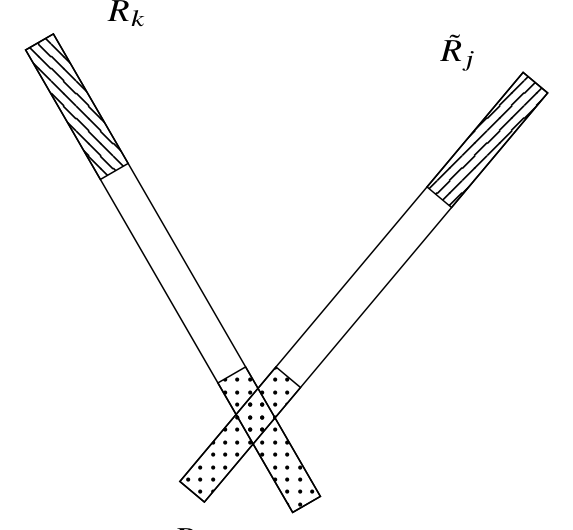
\includegraphics[width=0.36\textwidth]{figs/fig-5-1.png}
\caption{矩形与膨胀后的矩形.}
\label{fig:5.1}
\end{figure}

这在对足够大的 $N$ 时显然为假. 这意味着 $S_1$ 在 $L^p(\R^n)$（$n \geq 2$）上有界当且仅当 $p = 2$.

\section{Bochner--Riesz 算子: 球面求和}

Bochner--Riesz 算子，对 $\lambda > 0$ 定义为
\begin{align*}
  \widehat{T^{\lambda}f}(\xi)=(1-|\xi|^{2})_{+}^{\lambda}\widehat{f}(\xi),
\end{align*}
是球乘子的更光滑版本. 它们的核也可以用贝塞尔函数显式地求值:
\begin{align*}
  K_{\lambda}(x)=\pi^{-\lambda}\Gamma(1+\lambda)\left|x\right|^{-n/2-\lambda}J_{n/2+\lambda}(2\pi|x|),
\end{align*}
尽管这一事实对随后关于它们 $L^{p}$-有界性的讨论无关紧要.

若 $\lambda > (n-1)/2$（临界指数），则 $K_\lambda$ 可积，$T^\lambda$ 在每个 $L^p(\R^n)$（$1 \leq p \leq \infty$）上有界.

但当 $0 < \lambda < (n-1)/2$ 时，$K_\lambda$ 的衰减与奇异积分的 Calderón--Zygmund 理论相去甚远；事实上，一个明显的反例（$\widehat{f}$ 有界支集且 $|\xi| \leq 1$ 时 $\widehat{f}(\xi) \equiv 1$）表明 $T^\lambda$ 在区间
\begin{align*}
  \frac{2n}{n+1+2\lambda}<p<\frac{2n}{n-1-2\lambda}
\end{align*}
之外不可能有界.

但在这个区间内部，估计对径向函数 $f(|x|)$ 成立，对形如 $f(|x|)P_k(x)$ 的乘积也成立，其中 $P_k$ 是 $k$ 次球调和函数.

基于这些证据，人们提出了下面的猜想:

\begin{conjecture}\label{conj:5.5}
算子 $T^\lambda$ 在 $L^p(\R^n)$ 上有界，只要
\begin{align*}
  \frac{2n}{n+1+2\lambda}<p<\frac{2n}{n-1-2\lambda},\qquad 0<\lambda<\frac{n-1}{2}.
\end{align*}
\end{conjecture}

除 $n = 1$ 的情形外，该猜想只在二维被证明，本节的主要目的正是呈现其证明所涉及的思想.

\begin{theorem}\label{thm:5.6}
对 $0 < \lambda < 1/2$，算子 $T^\lambda$ 在
\begin{align*}
  \frac{4}{3+2\lambda}<p<\frac{4}{1-2\lambda}
\end{align*}
时于 $L^p(\R^2)$ 上有界.
\end{theorem}

乘子 $m_\lambda(\xi) = (1 - |\xi|^2)_{+}^\lambda$ 相当复杂，理解其性质的一个好策略是找出藏在 $m_\lambda$ 内部的 Calderón--Zygmund 理论的基本构件.

由于 $m_{\lambda}$ 是径向的，且在薄环上基本为常数，引入下列分解似乎合理:
\begin{align*}
  m_{\lambda}(\xi)=\sum_{k=0}^{\infty}(1-|\xi|^{2})_{+}^{\lambda}\phi_{k}(|\xi|),
\end{align*}
其中每个 $\phi_k$（$k \geq 1$）是支于区间 $[1-2^{-k}, 1-2^{-k+1}]$ 的光滑函数，满足 $|D^\alpha \phi_k| \leq C_\alpha 2^{k\alpha}$，$C_\alpha$ 与 $k$ 无关；且在区间 $1/2 \leq x \leq 1$ 上 $\sum_{k=1}^{\infty} \phi_k(x) \equiv 1$. 定义 $\phi_0 = 1 - \sum_{k=1}^{\infty} \phi_k$.

注意
\begin{align*}
  \phi_{j}(|\xi|)(1-|\xi|^{2})_{+}^{\lambda}\simeq 2^{-j\lambda}\phi_{j}(|\xi|),
\end{align*}
所以我们的问题化归为: 对 $j \to \infty$，得到乘子 $\phi_j(|\xi|)$ 范数增长的好的估计. 更精确地说，若我们能证明算子
\begin{align*}
  \widehat{T_{k}f}(\xi)=\phi_{k}(|\xi|)\widehat{f}(\xi)
\end{align*}
满足估计
\begin{align*}
  \left\|T_{k}f\right\|_{4}\lesssim k^{1/4}\left\|f\right\|_{4},\qquad f\in\mathcal{S}(\R^{2}),
\end{align*}
则定理 5.6 的证明将容易得到. 这是因为与估计 $\|T^k f\|_\infty \lesssim 2^{k/2}\|f\|_\infty$ 插值给出
\begin{align*}
  \left\|T_{k}f\right\|_{p}\lesssim k^{t/4}2^{k(1-t)/2}\left\|f\right\|_{p}.
\end{align*}
当 $1/p = t/4$ 且 $2 \leq p < 4/(1 - 2\lambda)$ 时，$1 - t < 2\lambda$，级数 $\sum_{j=1}^{\infty}2^{-j\lambda}j^{1/4}2^{j(1-t)/2}$ 收敛.

\begin{remark}\label{rem:5.7}
只要 $1 - t < 2\lambda$，上面的级数把幂 $j^{1/4}$ 换成 $j^\alpha$ 仍然收敛. 即，$T_k$ 在 $L^4(\R^2)$ 范数估计中的任何幂 $k^\alpha$ 都足以推出定理 5.6 的有效性，这为把定理推广到更一般的语境留出了灵活性.
\end{remark}

定理 5.6 将不过是下面命题的推论:

\begin{proposition}\label{prop:5.8}
设
\begin{align*}
  \widehat{S_{\delta}f}(\xi)=\phi(\delta^{-1}(1-|\xi|))\widehat{f}(\xi),
\end{align*}
其中 $0 < \delta < 1/2$，$\phi$ 是支于区间 $(-1,1)$ 的光滑函数. 存在与 $\delta$ 无关的有限常数 $C$，使
\begin{align*}
  \|S_{\delta}f\|_{4}\leq C\,|\log\delta|^{1/4}\|f\|_{4}
\end{align*}
对每个 Schwartz 类 $\mathcal{S}(\R^{2})$ 中的 $f$ 成立.
\end{proposition}

\begin{proof}
不失一般性，可以假设 $S_\delta$ 作用于其傅里叶变换 $\widehat{f}$ 支于角区域 $\{0 \leq \arg(\xi) \leq \pi/3\}$ 的函数 $f$ 上.

在单位圆上考虑光滑单位分解 $\psi_j$，$j = 1, 2, \ldots, [\delta^{-1/2}]$，使
\begin{align*}
  \psi_{j}(\theta)=\psi\bigl(\delta^{-1/2}\left(\theta-2\pi j\delta^{1/2}\right)\bigr),
\end{align*}
其中 $\psi$ 是支于单位区间的光滑函数（不失一般性，可设 $\delta^{-1/2}$ 是整数）.

有
\begin{align*}
  \widehat{S_{\delta}f}(|\xi|e^{i\theta})
  =\sum_{j=1}^{\delta^{-1/2}}\phi(\delta^{-1}(1-|\xi|))\psi_{j}(\theta)\widehat{f}(\xi)
  =\sum_{j}m_{j}(\xi)\widehat{f}(\xi)
  =\sum_{j}\widehat{T_{j}f}(\xi),
\end{align*}
\begin{align*}
  \int\Big|\sum_{j} T_{j} f\Big|^{4}\mathrm{d}x
  &=\int\Big|\sum_{j,k}T_{j} f(x)\,T_{k} f(x)\Big|^{2}\mathrm{d}x
  =\int\Big|\sum_{j,k}\widehat{T_{j} f}*\widehat{T_{k} f}(\xi)\Big|^{2}\mathrm{d}\xi\\
  &\lesssim\sum_{j,k}\int|\widehat{T_{j} f}*\widehat{T_{k} f}(\xi)|^{2}\mathrm{d}\xi
  =\int\Big(\sum_{j}|T_{j} f(x)|^{2}\Big)^{2}\mathrm{d}x,
\end{align*}
其中上述不等式中的关键点是: 集合族 $\supp(\widehat{T_j f}) + \supp(\widehat{T_k f})$ 具有与 $\delta$ 无关的有限重叠.

接下来，利用逐点估计
\begin{align*}
  \Big(\sum_{j}|T_{j}f(x)|^{2}\Big)^{1/2}
  \leq\Big(\sum_{j}|T_{2j}f(x)|^{2}\Big)^{1/2}
  +\Big(\sum_{j}|T_{2j+1}f(x)|^{2}\Big)^{1/2},
\end{align*}
并注意到右端两项具有相同的范数.

关于第一项，$m_{2j}(\xi)$ 的支集基本垂直于水平轴，我们可以找到一列沿竖直方向均匀分布的水平带 $E_j$，使
\begin{align*}
  \supp(m_{2j})\subset E_{2j}.
\end{align*}

\begin{figure}[htbp]
\centering
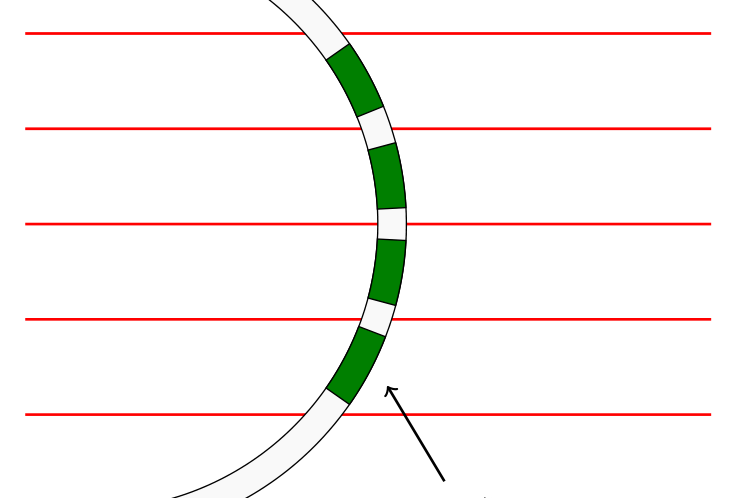
\includegraphics[width=0.44\textwidth]{figs/fig-5-2.png}
\caption{$G$-函数.}
\label{fig:5.2}
\end{figure}

于是 $m_{2j}(\xi) = m_{2j}(\xi)E_{2j}(\xi)$. 定义
\begin{align*}
  \widehat{P_{2j}f}(\xi)=E_{2j}(\xi)\widehat{f}(\xi),
\end{align*}
有
\begin{align*}
  \Big(\sum_{j}|T_{2j}f(x)|^{2}\Big)^{1/2}
  =\Big(\sum_{j}|T_{2j}P_{2j}f(x)|^{2}\Big)^{1/2}.
\end{align*}

一个初等的分部积分论证给出 $T_0$ 的核 $K_0$ 满足: 对每对整数 $\alpha, \beta \geq 0$，存在与 $\delta$ 无关的有限常数 $C_{\alpha,\beta}$，使
\begin{align*}
  |K_{0}(x,y)|\leq C_{\alpha,\beta}\delta^{3/2}|\delta x|^{-\alpha}|\delta^{1/2}y|^{-\beta},
\end{align*}
其中 $(x, y)$ 是 $\R^2$ 中的标准直角坐标.

于是算子 $T_{0}$ 逐点地被核为
\begin{align*}
  C\sum_{n=0}^{\infty}2^{-n}\frac{1}{\mu(R_{n}^{0})}\chi_{R_{n}^{0}}(x,y)
\end{align*}
的正算子控制，其中
\begin{align*}
  R_{n}^{0}=\{(x,y):|x|\leq 2^{n}\delta^{-1},\ |y|\leq 2^{n}\delta^{-1/2}\},
\end{align*}
$C$ 是与 $\delta$ 无关的适当常数. 用适当的旋转，对每一块 $T_{j}$ 得到类似的控制.

由于衰减 $2^{-n}$，只须证明: 对每个 $n$，函数
\begin{align*}
  \Big(\sum_{j}\Big|\frac{1}{\mu(R_{n}^{2j})}\chi_{R_{n}^{2j}}*P_{2j}f(x)\Big|^{2}\Big)^{1/2}
\end{align*}
的 $L^{4}$-范数以 $C|\log\delta|^{1/4}\|f\|_{4}$ 为界.

为看出这一点，取 $L^2(\R^2)$ 中的 $\omega \geq 0$，考虑积分
\begin{align*}
  \sum_{j}\int\Big|\frac{1}{\mu(R_{n}^{2j})}\chi_{R_{n}^{2j}}*P_{2j}f(x)\Big|^{2}\omega(x)\,\mathrm{d}x
  &\lesssim\sum_{j}\int|P_{2j}f(y)|^{2}\frac{1}{\mu(R_{n}^{2j})}\chi_{R_{n}^{2j}}*\omega(y)\,\mathrm{d}y\\
  &\lesssim\sum_{j}\int|P_{2j}f(y)|^{2}M\omega(y)\,\mathrm{d}y\\
  &\qquad\leq\Big\|\Big(\sum_{j}|P_{2j}f|^{2}\Big)^{1/2}\Big\|_{4}^{2}\|M\omega\|_{2},
\end{align*}
其中 $M$ 是第 3 章中对应离心率 $N = \delta^{-1/2}$ 矩形的 Kakeya 极大函数. 于是
\begin{align*}
  \Big\|\Big(\sum_{j}|T_{2j}f|^{2}\Big)^{1/2}\Big\|_{4}^{2}
  &\leq\sup_{\|\omega\|_{2}=1}\int\sum_{j}|T_{2j}f(x)|^{2}\omega(x)\,\mathrm{d}x\\
  &\lesssim|\log\delta|^{1/2}\Big\|\Big(\sum_{j}|P_{2j}f|^{2}\Big)^{1/2}\Big\|_{4}^{2},
\end{align*}
而命题将是下面引理的推论:
\end{proof}

\begin{lemma}\label{lem:5.9}
在 $\R^n$ 中，考虑格 $\mathcal{L} = \{Q_\nu\}_{\nu \in \Z^n}$. 即，平行多面体 $Q_\nu$ 全等、内部两两不交，且 $\R^n = \bigcup_\nu Q_\nu$.

对每个 $\nu \in \Z^n$ 定义算子
\begin{align*}
  \widehat{P_{\nu}f}(\xi)=Q_{\nu}(\xi)\widehat{f}(\xi)
\end{align*}
以及平方函数
\begin{align*}
  G f(x)=\Big(\sum_{\nu}|P_{\nu}f(x)|^{2}\Big)^{1/2}.
\end{align*}
则对每个 $s > 1$，存在有限常数 $C_s$，使对每个局部可积函数 $\omega \geq 0$ 与每个 $f \in \mathcal{S}(\R^n)$,
\begin{align*}
  \int_{\R^{n}}[G f(x)]^{2}\omega(x)\,\mathrm{d}x
  \leq C_{s}\int_{\R^{n}}|f(x)|^{2}A_{s}\omega(x)\,\mathrm{d}x,
\end{align*}
其中 $A_{s}\omega(x)=[M\omega^{s}(x)]^{1/s}$，$M$ 表示 $\R^{n}$ 中的强极大函数.
\end{lemma}

\begin{proof}
用方便的膨胀，不失一般性可设 $\mathcal{L}$ 是单位格，即 $Q_\nu$ 是以点 $\nu \in \Z^n$ 为中心的单位方体.

设 $\psi$ 是紧支集光滑函数，使 $\psi \equiv 1$ 于 $Q_0$ 内部. 对每个 $y \in Q_0$，考虑由
\begin{align*}
  m_{y}(z)=\sum_{\nu}\exp(2\pi i\nu\cdot y)\,\psi(z-\nu)
\end{align*}
给出的傅里叶乘子. 核 $\mu_y = \widehat{m}_y$ 是总变差有限的测度，对 $y \in Q_0$ 一致. 更精确地,
\begin{align*}
  \mu_{y}=\sum_{\nu}\widehat{\psi}(y+\nu)\,\delta_{y+\nu},
\end{align*}
其中 $\delta_{x}$ 表示 Dirac $\delta$ 函数. 于是
\begin{align*}
  |\mu_{y}*f(x)|^{2}\lesssim\sum_{\nu}(1+|\nu|)^{2n}\left|\widehat{\psi}(y+\nu)\right|^{2}|f(x-y-\nu)|^{2},
\end{align*}
利用 $\psi$ 速降的事实，对足够大的 $N$ 有
\begin{align*}
  \int_{\R^{n}}|\mu_{y}*f(x)|^{2}\omega(x)\,\mathrm{d}x
  \leq C_{N}\sum_{\nu}(1+|\nu|)^{2n-N}\int_{\R^{n}}|f(x)|^{2}\omega(x+y+\nu)\,\mathrm{d}x.
\end{align*}
选取 $N \geq 4n$，得
\begin{align*}
  \int_{Q_{0}}\int_{\R^{n}}&|\mu_{y}*f(x)|^{2}\omega(x)\,\mathrm{d}x\,\mathrm{d}y\\
  &\leq C_{N}\sum_{\nu}(1+|\nu|)^{2n-N}\int_{\R^{n}}|f(x)|^{2}\Big(\int_{Q_{0}}\omega(x+y+\nu)\,\mathrm{d}y\Big)\mathrm{d}x\\
  &\lesssim\int_{\R^{n}}|f(x)|^{2}M\omega(x)\,\mathrm{d}x,
\end{align*}
其中 $M$ 是 Hardy--Littlewood 极大函数.

但另一方面，若 $\widehat{T_{\nu}f}(\xi)=\psi(\xi-\nu)\widehat{f}(\xi)$，则有
\begin{align*}
  \mu_{y}*f(x)=\sum_{\nu}\exp(2\pi i\nu\cdot y)\,T_{\nu}f(x),
\end{align*}
以及
\begin{align*}
  \int_{Q_{0}}\int_{\R^{n}}\left|\mu_{y}*f(x)\right|^{2}\omega(x)\,\mathrm{d}x\,\mathrm{d}y
  =\sum_{\nu}\int_{\R^{n}}\left|T_{\nu}f(x)\right|^{2}\omega(x)\,\mathrm{d}x,
\end{align*}
由此得到所求的估计:
\begin{align*}
  \sum_{\nu}\int_{\R^{n}}&|P_{\nu}f(x)|^{2}\omega(x)\,\mathrm{d}x
  =\sum_{\nu}\int_{\R^{n}}|P_{\nu}T_{\nu}f(x)|^{2}\omega(x)\,\mathrm{d}x\\
  &\lesssim C_{s}\sum_{\nu}\int_{\R^{n}}|T_{\nu}f(x)|^{2}A_{s}\omega(x)\,\mathrm{d}x
  \lesssim C_{s}\int_{\R^{n}}|f(x)|^{2}A_{s}\omega(x)\,\mathrm{d}x.
\end{align*}
\end{proof}

\begin{remark}\label{rem:5.10}
引理~\ref{lem:5.9} 有一个更强的（无权重）版本，其中格被换成更一般的、各边平行于坐标轴的两两不交平行多面体族. 一维情形的证明由 J.~L.~Rubio de Francia \cite{b123} 获得，任意维数由 J.-L.~Journé \cite{b119} 获得.
\end{remark}

\section{向量值不等式}

现在考虑 Bochner--Riesz 算子的膨胀 $T_{R}^{\lambda}$:
\begin{align*}
  \widehat{T_{R}^{\lambda}f}(\xi)=(1-|\xi|^{2}/R^{2})_{+}^{\lambda}\widehat{f}(\xi),
\end{align*}
并设 $\{R_j\}$ 是正数的任何序列. 则有定理 5.6 的向量值版本.

\begin{theorem}\label{thm:5.11}
在 $\R^2$ 中，给定 $\lambda > 0$ 与 $4/(3+2\lambda) < p < 4/(1-2\lambda)$，存在有限常数 $C_{p,\lambda}$，使
\begin{align*}
  \left\|\Big(\sum_{j}|T_{R_{j}}^{\lambda}f_{j}|^{2}\Big)^{1/2}\right\|_{p}
  \leq C_{p,\lambda}\left\|\Big(\sum_{j}|f_{j}|^{2}\Big)^{1/2}\right\|_{p}.
\end{align*}
\end{theorem}

\begin{proof}
如定理 5.6 的证明，可以把估计化归为乘子支于薄环上的情形. 假设 $\phi: \R \to \R$ 是支于 $[-1,+1]$ 的光滑函数，定义
\begin{align*}
  \widehat{S_{j}^{\delta}f}(\xi)&=\phi(\delta^{-1}(1-|\xi|/R_{j}))\widehat{f}(\xi),\\
  \widehat{T_{j}^{n}f}(\xi)&=\psi_{n}(\arg(\xi))\widehat{S_{j}^{\delta}f}(\xi)=m_{j,n}(\xi)\widehat{f}(\xi),
\end{align*}
其中 $\{\psi_{n}\}$ 是命题 5.8 中引入的光滑角向单位分解.

不失一般性，还可以假设
\begin{align*}
  \supp(\widehat{f_{j}})\subset\{0\leq\arg(\xi)\leq\pi/3\},\qquad \text{对每个 } j.
\end{align*}
回忆 $\psi_n$ 支于 $|\theta-2\pi n/N| \leq 2\pi/N$，其中 $N = \delta^{-1/2}$（不失一般性可视为整数）. 这意味着 $m_{j,n}(\xi)$ 支于尺寸为 $R_j \delta \times R_j \delta^{1/2}$、方向为 $2\pi n/N$ 的``矩形''上.

证明分三步:

(a) 与定理 5.6 所用类似的论证允许把证明化归为不等式
\begin{align*}
  \left\|\Big(\sum_{j}|S_{j}^{\delta}f_{j}|^{2}\Big)^{1/2}\right\|_{4}
  \leq C|\log\delta|^{\alpha}\left\|\Big(\sum_{j}|f_{j}|^{2}\Big)^{1/2}\right\|_{4}.
\end{align*}

(b) 借助乘子的适当分解与若干几何论证，我们证明
\begin{align*}
  \left\|\Big(\sum_{j}|S_{j}^{\delta}f_{j}|^{2}\Big)^{1/2}\right\|_{4}
  \leq C|\log\delta|\left\|\Big(\sum_{j,n}|T_{j}^{n}f_{j}|^{2}\Big)^{1/2}\right\|_{4}.
\end{align*}

(c) 对 $T_j^n$ 的核的估计，连同引理 5.9 与定理 3.7，给出
\begin{align*}
  \left\|\Big(\sum_{j,n}|T_{j}^{n} f_{j}|^{2}\Big)^{1/2}\right\|_{4}
  \leq C|\log\delta|^{\beta}\left\|\Big(\sum_{j}|f_{j}|^{2}\Big)^{1/2}\right\|_{4}.
\end{align*}

第 (a) 部分留给读者.

关于第 (b) 部分，首先在每个 $|\log_2 \delta|$ 个相邻区间中只选出一个二进区间 $2^k < R \leq 2^{k+1}$，并且只允许 (b) 左端那些 $R_j$ 落在所选区间中的指标 $j$ 出现. 同时，对每四个相邻指标 $n$ 只取一个 $T_j^n$，并且只取那些支于角扇形 $\{0 \leq \arg(\xi) \leq \pi/3\}$ 者. 所有这些操作都会给不等式 (b) 贡献因子 $C|\log \delta|$.

(b) 的左端小于下面量的四次根的二倍:
\begin{align*}
  \sum_{R_{j}\leq R_{k}}\int\left|\Big(\sum_{n}T_{j}^{n} f_{j}\Big)\Big(\sum_{m}T_{k}^{m} f_{k}\Big)\right|^{2}.
\end{align*}
可以区分两类点对 $(j, k)$: 或 $R_j \leq R_k \leq 2R_j$，或 $R_j \leq \delta R_k$. 记上述和的两部分为 $\sum_{\mathrm{I}}$ 与 $\sum_{\mathrm{II}}$. 有
\begin{align*}
  \sum_{\mathrm{I}}
  =\sum_{\mathrm{I}}\int\left|\sum_{n,m}(\widehat{T_{j}^{n}f_{j}})\ast(\widehat{T_{k}^{m}f_{k}})\right|^{2}
  \leq 4\sum_{\mathrm{I}}\int\left|\sum_{n\leq m}\widehat{T_{j}^{n}f_{j}}\ast\widehat{T_{k}^{m}f_{k}}\right|^{2},
\end{align*}
一个简单的几何论证表明，对固定的 $j$ 与 $k$，对不同对 $n \leq m$，$\widehat{T_{j}^{n} f_{j}} * \widehat{T_{k}^{m} f_{k}}$ 的支集互不相交. 因此,
\begin{align*}
  \sum_{\mathrm{I}}\leq 4\int\sum_{\mathrm{I}}\sum_{n\leq m}|\widehat{T_{j}^{n}f_{j}}*\widehat{T_{k}^{m}f_{k}}|^{2}\leq 4A,
\end{align*}
其中
\begin{align*}
  A=\Big\|\Big(\sum_{j,n}|T_{j}^{n} f_{j}|^{2}\Big)^{1/2}\Big\|_{4}^{4}.
\end{align*}
其次注意，当 $(j,k)$ 属于情形 $\Sigma_{\mathrm{II}}$ 时，$R_{j} \leq \delta R_{k}$，且卷积
\begin{align*}
  \widehat{T_{j}^{n_{1}}f_{j}}*\widehat{T_{k}^{m_{1}}f_{k}},\qquad
  \widehat{T_{j}^{n_{2}}f_{j}}*\widehat{T_{k}^{m_{2}}f_{k}}
\end{align*}
的支集在 $m_1 \neq m_2$ 时不交. 则
\begin{align*}
  \sum_{\mathrm{II}}
  &=\sum_{\mathrm{II}}\int\Big|\sum_{m}\Big(\sum_{n}T_{j}^{n}f_{j}\Big)T_{k}^{m}f_{k}\Big|^{2}\\
  &\leq\Big[\int\Big(\sum_{j}\Big|\sum_{n}T_{j}^{n}f_{j}\Big|^{2}\Big)^{1/2}\Big]^{1/2}
   \cdot\Big[\int\Big(\sum_{k,m}|T_{k}^{m}f_{k}|^{2}\Big)^{2}\Big]^{1/2}
  \leq\sqrt{2}\left[\sum_{\mathrm{I}}+\sum_{\mathrm{II}}\right]^{1/2}A^{1/2},
\end{align*}
这就推出 (b).

为证明第 (c) 部分，首先注意对每个固定的 $j$，可以选取如引理 5.9 那样的矩形网格，使每个乘子 $m_{j,n}(\xi)$ 支于网格中的某个矩形 $Q_{j}^{n}$ 内.

若 $\widehat{P_j^n f} = Q_j^n\cdot\widehat{f}$ 是相应的傅里叶乘子，则有恒等式
\begin{align*}
  T_{j}f_{j}=T_{j}^{n}P_{j}^{n}f_{j}.
\end{align*}
此外，分部积分论证（如定理 5.6 中）表明 $T_j^n$ 的核被
\begin{align*}
  C\sum_{\nu=0}^{\infty}2^{-\nu}\frac{1}{|R_{\nu,j}^{n}|}R_{\nu,j}^{n}(x)
\end{align*}
控制，其中 $R_{\nu,j}^n$ 是尺寸 $2^\nu\delta^{-1} \times 2^\nu\delta^{-1/2}$、方向角 $2\pi\delta^{1/2}n$ 的矩形，$C$ 与 $n$、$j$ 和 $\delta > 0$ 无关.

于是，为估计 $A$，需要对 $\nu$ 一致地估计
\begin{align*}
  \Big[\sum_{j,n}\Big(\frac{1}{|R_{\nu,j}^{n}|}R_{\nu,j}^{n}*|P_{j}^{n}f_{j}|\Big)^{2}\Big]^{1/2}
\end{align*}
的 $L^{4}$-范数. 若 $w \geq 0$ 属于 $L^2(\R^2)$，有
\begin{align*}
  &\sum_{j,n}\int\left[\frac{1}{\left|R^{n}_{\nu,j}\right|}R^{n}_{\nu,j}*|P^{n}_{j} f_{j}|\right]^{2}\omega(x)\,\mathrm{d}x
  \leq\sum_{j,n}\int|P^{n}_{j} f_{j}(y)|^{2}\left[\frac{1}{\left|R^{n}_{\nu,j}\right|}R^{n}_{\nu,j}*\omega(y)\right]\mathrm{d}y\\
  &\quad\leq\sum_{j,n}\int|P^{n}_{j} f_{j}(y)|^{2}M\omega(y)\,\mathrm{d}y
  \leq C_{s}\sum_{j}\int|f_{j}(y)|^{2}A_{s}(M\omega)(y)\,\mathrm{d}y\\
  &\quad\leq\widetilde{C}_{s}\left\|\Big(\sum_{j}|f_{j}|^{2}\Big)^{1/2}\right\|_{4}^{2}\|M\omega\|_{2}
  \leq C\left|\log\delta\right|^{1/2}\|\omega\|_{2}\left\|\Big(\sum_{j}|f_{j}|^{2}\Big)^{1/2}\right\|_{4}^{2},
\end{align*}
其中再次用到了引理 5.9 与第 3 章 Kakeya 极大函数的估计.
\end{proof}

\section{一个角平方函数}

在 $\R^2$ 中，考虑角 $\omega_j = 2\pi j/N$，$j = 0,1,\ldots,N-1$，区域
\begin{align*}
  \Delta_{j}=\{\xi:\omega_{j}\leq\arg(\xi)\leq\omega_{j+1}\},
\end{align*}
傅里叶乘子
\begin{align*}
  \widehat{S_{j}f}(\xi)=\Delta_{j}(\xi)\widehat{f}(\xi)
\end{align*}
以及相伴的平方函数
\begin{align*}
  G(f)(x)=\left(\sum_{j}\left|S_{j}f(x)\right|^{2}\right)^{1/2}.
\end{align*}

\begin{theorem}\label{thm:5.12}
存在与 $N$ 无关的常数 $a$ 与 $C$，使
\begin{align*}
  \left\|G(f)\right\|_{4}\leq C\left[\log N\right]^{a}\left\|f\right\|_{4}
\end{align*}
对每个 Schwartz 类 $\mathcal{S}(\R^{2})$ 中的 $f$ 成立.
\end{theorem}

设 $\{\psi_j\}$ 是如定理 5.11 中的角截断函数，使 $\psi_j \equiv 1$ 于 $\Delta_j$，$\supp(\psi_j) \subset \Delta_{j-1} \cup \Delta_j \cup \Delta_{j+1}$，写
\begin{align*}
  \widehat{\widetilde{S}_{j}f}(\xi)=\psi_{j}(\xi)\widehat{f}(\xi),\qquad
  \widetilde{G}f(x)=\Big(\sum_{j}|\widetilde{S}_{j}f(x)|^{2}\Big)^{1/2}.
\end{align*}
于是，借助第 3 章 Kakeya 极大函数的估计，定理 5.12 将是下面命题的推论.

\begin{proposition}\label{prop:5.13}
存在与 $N$ 无关的有限常数 $a$ 与 $C$，使:
\begin{align*}
  \|\widetilde{G}(f)\|_{4}\leq C\left[\log N\right]^{a}\|f\|_{4}.
\end{align*}
\end{proposition}

设 $\{\phi_n\}$ 是满足 $\supp(\phi_n) \subset (2^{n-1}, 2^{n+1})$ 与 $|D_x^\alpha \phi_n| \leq C_\alpha 2^{-n\alpha}$ 的光滑函数，定义
\begin{align*}
  \widehat{\widetilde{S}_{j,n}f}(\xi)=\phi_{n}(|\xi|)\psi_{j}(\xi)\widehat{f}(\xi),\qquad
  \widetilde{G}_{n}f(x)=\Big(\sum_{j}|\widetilde{S}_{j,n}f(x)|^{2}\Big)^{1/2}.
\end{align*}
于是，第一步我们将证明估计
\begin{align*}
  \|\widetilde{G}_{n}f\|_{4}\leq C\left[\log N\right]^{a}\|f\|_{4},
\end{align*}
常数 $C$ 与 $a$ 与 $n$ 和 $N$ 无关. 但一个简单的膨胀论证表明，只须证明 $n = 1$ 的情形.

第二步，我们将把这些估计合在一起得到命题的证明. 还要注意到，不失一般性，可以假设函数 $f$ 的傅里叶变换支于区域
\begin{align*}
  \{\xi:0\leq\arg(\xi)\leq\pi/4\}.
\end{align*}
我们必须计算
\begin{align*}
  \|\widetilde{G}_{1}f\|_{4}^{4}
  =\sum_{j,k}\int_{\R^{2}}\left|\widetilde{S}_{j}f(x)\widetilde{S}_{k}f(x)\right|^{2}\mathrm{d}x
  =\sum_{|j-k|\leq 4}(\cdots)+\sum_{|j-k|>4}(\cdots)=\mathrm{I}+\mathrm{II}.
\end{align*}
接着把 $\phi_1(|\xi|)\psi_j(\xi)$ 的支集进一步分解成 $N^{1/2}$ 个部分 $\Delta_j^\alpha$，$\alpha = 1, \ldots, N^{1/2}$，其中
\begin{align*}
  \Delta_{j}^{\alpha}=\left\{\xi\in\supp(\phi_{1}\cdot\psi_{j}):\alpha N^{-1/2}\leq|\xi|-1\leq(\alpha+1)N^{-1/2}\right\}
\end{align*}
（同样，不失一般性可设 $N^{1/2}$ 是整数）. 当 $|j - k| \geq 4$ 时，集合 $\Delta_j^\alpha + \Delta_k^\beta$ 的重叠有界，且对 $N$ 一致.

于是，再次用 Plancherel 定理，得
\begin{align*}
  \mathrm{II}
  &\leq\sum_{|j-k|\geq 4}\sum_{\alpha,\beta}\int_{\R^{2}}|\widetilde{S}_{j}^{\alpha}f(x)\;\widetilde{S}_{k}^{\beta}f(x)|^{2}\mathrm{d}x
  \leq\left\|\Big(\sum_{j,\alpha}|\widetilde{S}_{j}^{\alpha}f|^{2}\Big)^{1/2}\right\|_{4}^{4},
\end{align*}
其中
\begin{align*}
  \widehat{\widetilde{S}_{j}^{\alpha}f}(\xi)=\phi_{1}(|\xi|)\psi_{j}(\xi)\eta_{\alpha}(|\xi|)\widehat{f}(\xi),
\end{align*}
$\eta_\alpha$ 是适应的光滑截断族，即在 $\phi_1\psi_j$ 的支集上有 $\sum_\alpha \eta_\alpha(|\xi|) \equiv 1$，且
\begin{align*}
  \supp\eta_{\alpha}\subset(1+\alpha N^{-1/2},1+(\alpha+2)N^{-1/2}),\qquad
  |D_{x}^{m}\eta_{\alpha}|\leq C_{m}N^{m/2}.
\end{align*}
注意
\begin{align*}
  \mathrm{I}
  &\leq\int\left(\sum_{j}|\widetilde{S}_{j} f|^{4}\right)
  \leq\int\left(\sum_{j}|\widetilde{S}_{j} f|^{2}\right)\cdot\left(\sup_{j}|\widetilde{S}_{j} f(x)|^{2}\right)\mathrm{d}x\\
  &\leq\left(\int\sum_{j,k}|\widetilde{S}_{j} f(x)\widetilde{S}_{k} f(x)|^{2}\mathrm{d}x\right)^{1/2}\left[\int|M_{N} f(x)|^{4}\right]^{1/2}\\
  &\leq\frac{1}{2}\varepsilon\left(\mathrm{I}+\mathrm{II}\right)+\frac{1}{2}\frac{1}{\varepsilon}C\left(\log N\right)^{a}\|f\|_{4}^{4}
\end{align*}
对每个 $\varepsilon > 0$ 成立. 因此，适当地选取 $\varepsilon$，只须证明估计
\begin{align*}
  \mathrm{II}\lesssim[\log N]^{a}\left\|{f}\right\|_{4}^{4}.
\end{align*}
为此，设 $\omega \geq 0$ 满足 $\|\omega\|_2 = 1$，考虑积分
\begin{align*}
  \sum_{j,\alpha}\int|\widetilde{S}_{j}^{\alpha}f(x)|^{2}\omega(x)\,\mathrm{d}x
  &=\sum_{\alpha=1}^{N^{1/2}}\int\Big|\sum_{j}\widetilde{S}_{j}^{\alpha}f(x)\Big|^{2}\omega(x)\,\mathrm{d}x\\
  &=\sum_{\alpha=1}^{N^{1/2}}\sum_{\tau=0}^{N^{1/2}}\int\Big|\sum_{j=\tau N^{1/2}}^{(\tau+1)N^{1/2}}\widetilde{S}_{j}^{\alpha}f(x)\Big|^{2}\omega(x)\,\mathrm{d}x\\
  &=\sum_{\alpha=1}^{N^{1/2}}\sum_{\tau=0}^{N^{1/2}}\int\Big|\sum_{j=\tau N^{1/2}}^{(\tau+1)N^{1/2}}\widetilde{S}_{j}^{\alpha}E_{j}^{\alpha}f(x)\Big|^{2}\omega(x)\,\mathrm{d}x,
\end{align*}
其中 $E_j^\alpha$ 是两两不交的矩形，平行于 $\Delta_j$ 的角平分线，尺寸约为 $N^{-1/2} \times N^{-1}$，满足 $E_j^\alpha \supset \phi_1\psi_j\eta_\alpha$；算子 $E_j^\alpha$ 由公式
\begin{align*}
  \widehat{E_{j}^{\alpha}f}(\xi)=E_{j}^{\alpha}(\xi)\widehat{f}(\xi)
\end{align*}
定义，这里我们再次使用了以同一符号 $E_{j}^{\alpha}$ 表示集合、其示性函数以及相伴傅里叶乘子的约定.

我们现在可以应用引理 5.9:
\begin{align*}
  \sum_{j,\alpha}\int\left|\widetilde{S}_{j}^{\alpha}f(x)\right|^{2}\omega(x)\,\mathrm{d}x
  &=\sum_{j,\alpha}\int\left|\widetilde{S}_{j}^{\alpha}E_{j}^{\alpha}f(x)\right|^{2}\omega(x)\,\mathrm{d}x\\
  &\lesssim\sum_{\alpha=1}^{N^{1/2}}\sum_{\tau=0}^{N^{1/2}}\int|Q_{\alpha}^{\tau}f(x)|^{2}M_{N}\omega(x)\,\mathrm{d}x,
\end{align*}
因为如定理 5.11，$\widetilde{S}_{j}^{\alpha}$ 的核被一个和
\begin{align*}
  C\sum_{\nu=0}^{\infty}2^{-\nu}\frac{1}{|R_{j,n}^{\alpha}|}R_{j,n}^{\alpha}(x)
\end{align*}
控制，其中 $R_{j,n}^{\alpha}$ 是 $j$ 方向上离心率 $N^{1/2}$ 的矩形. 这里对每个 $\alpha, \tau = 1, \ldots, N^{1/2}$，$Q_{\alpha}^{\tau}$ 现在是边长 $\sim N^{-1/2}$ 的正方形，族 $\{Q_{\alpha}^{\tau}\}$ 有普适有界的重叠.

再应用一次引理 5.9，连同 Kakeya 极大函数的已知估计，即得所求不等式.

为结束证明，把``二进''截断函数 $\phi_n$ 的指标按 $\bmod[\log_2 N]$ 分成剩余类，把方向指标 $j$ 按 $\bmod(4)$ 分成类，并应用定理 5.11 的同样方法.

\section{极大 Bochner--Riesz 算子: 逐点收敛}

对 $\lambda > 0$，极大函数
\begin{align*}
  T_{*}^{\lambda}f(x)=\sup_{R>0}|T_{R}^{\lambda}f(x)|,
\end{align*}
其中 $T_{R}^{\lambda}f(\xi)=(1-|\xi|^{2}/R^{2})_{+}^{\lambda}\widehat{f}(\xi)$，控制着当 $R$ 趋于无穷时 $T_{R}^{\lambda}f(x)$ 到 $f(x)$ 的几乎处处收敛.

利用单位球在边界附近厚度 $\delta$ 的冠状环的标准分解（$\delta = 2^{-k}$，$k = 1, 2, \ldots$），$T_*$ 的 $L^p$-有界性化归为对
\begin{align*}
  S_{*}^{\delta}f(x)=\sup_{R>0}|S_{R}^{\delta}f(x)|
\end{align*}
得到好的估计，其中
\begin{align*}
  \widehat{S_{R}^{\delta}f}(\xi)=\phi(|\xi|,R)\widehat{f}(\xi),
\end{align*}
$\phi$ 是任何满足下列条件的光滑函数:
\begin{align*}
  \supp\phi(\cdot,t)\subset(t-t\delta,t+t\delta),\qquad
  |D_{r}^{\alpha}\phi(r,t)|\leq C_{\alpha}(t\delta)^{-\alpha},
\end{align*}
\begin{align*}
  D_{t}\phi(r,t)=\psi(r,t)(t\delta)^{-1},
\end{align*}
\begin{align*}
  \supp\psi(r,t)\subset(t-t\delta,t+t\delta),\qquad
  |D_{r}^{\alpha}\psi(r,t)|\leq C_{\alpha}(t\delta)^{-\alpha}.
\end{align*}
一个例子是
\begin{align*}
  \phi(|\xi|,t)=\varphi\left(\frac{|\xi|-t}{\delta t}\right),
\end{align*}
其中 $\varphi$ 是支于 $(-1,+1)$ 的光滑函数.

\begin{theorem}\label{thm:5.14}
$S_{*}^{\delta}$ 在 $L^2(\R^n)$ 上有界.
\end{theorem}

\begin{corollary}\label{cor:5.15}
当 $\lambda > 0$ 时，对每个 $f \in L^2(\R^n)$，$\lim_{R \to \infty} T_R^\lambda f(x) = f(x)$ 几乎处处成立.
\end{corollary}

\begin{proof}[定理~\ref{thm:5.14} 的证明]
有
\begin{align*}
  (S_{R}^{\delta}f(x))^{2}
  =\int_{0}^{R}\frac{\mathrm{d}}{\mathrm{d}t}(S_{t}^{\delta}f(x))^{2}\,\mathrm{d}t
  =2\int_{0}^{R}S_{t}^{\delta}f(x)\cdot\frac{\mathrm{d}}{\mathrm{d}t}(S_{t}^{\delta}f(x))\,\mathrm{d}t,
\end{align*}
由此得估计
\begin{align*}
  S_{*}^{\delta}f(x)
  &\leq\delta^{-1/2}\Big(\int_{0}^{\infty}\left|S_{t}^{\delta}f(x)\right|^{2}\frac{\mathrm{d}t}{t}\Big)^{1/2}
   +\delta^{1/2}\Big(\int_{0}^{\infty}\left|\frac{\mathrm{d}}{\mathrm{d}t}S_{t}^{\delta}f(x)\right|^{2}t\,\mathrm{d}t\Big)^{1/2}\\
  &=\delta^{-1/2}G_{1}^{\delta}f(x)+\delta^{1/2}G_{2}^{\delta}f(x),
\end{align*}
以及
\begin{align*}
  \int_{\R^{n}}|G_{1}^{\delta}f(x)|^{2}\,\mathrm{d}x
  =\int_{\R^{n}}\Big(\int_{0}^{\infty}|\phi(|\xi|,t)|^{2}\frac{\mathrm{d}t}{t}\Big)|\widehat{f}(\xi)|^{2}\,\mathrm{d}\xi
  \leq C\delta\|f\|_{2}^{2},
\end{align*}
\begin{align*}
  \int_{\R^{n}}|G_{2}^{\delta}f(x)|^{2}\,\mathrm{d}x
  =\int_{\R^{n}}\Big(\int_{0}^{\infty}|\psi(|\xi|,t)|^{2}\frac{\mathrm{d}t}{t}\Big)|\widehat{f}(\xi)|^{2}\,\mathrm{d}\xi
  \leq C\delta^{-1}\|f\|_{2}^{2}.
\end{align*}
\end{proof}

在维数 $n = 2$ 中，定理 5.14 容许若干改进.

首先考虑 $\{R_j\}$ 是缺项的，即对每个 $j$ 有 $R_{j+1}/R_j > \rho > 1$，并考虑相伴的极大算子
\begin{align*}
  M_{*}^{\lambda}f(x)=\sup_{j}|T_{R_{j}}^{\lambda}f(x)|.
\end{align*}
则有:

\begin{theorem}\label{thm:5.16}
对 $0 < \lambda < 1/2$，极大算子 $M_{*}^{\lambda}$ 在 $L^p(\R^2)$ 上有界，当且仅当 $4/(3+2\lambda) < p < 4/(1-2\lambda)$.
\end{theorem}

\begin{proof}
用定理 5.11 引入的记号与类似论证，只须证明估计
\begin{equation}\label{eq:5.3}
  \left\|\Big(\sum_{j}|S_{j}^{\delta}f|^{2}\Big)^{1/2}\right\|_{4}
  \leq C\left|\log\delta\right|^{a}\|f\|_{4}
\end{equation}
对某个与 $\delta > 0$ 无关的有限常数 $a$ 与 $C$ 成立，其中
\begin{align*}
  \widehat{S_{j}^{\delta}f}(\xi)=\phi(\delta^{-1}\left(1-|\xi|/R_{j}\right))\widehat{f}(\xi).
\end{align*}
注意，不失一般性，只须对傅里叶变换 $\widehat{f}$ 支于角 $\{\xi : 0 \leq \arg(\xi) \leq \pi/3\}$ 的函数 $f$ 证明 \eqref{eq:5.3}.

由于当 $1 < \rho \leq 2$ 时，每个二进区间 $[2^l, 2^{l+1}]$ 至多含 $1 + |\log \delta|$ 个缺项集 $\{R_j\}$ 的元素，我们也可以（再次不失一般性）假设 $\rho \geq 2$，从而每个二进区间至多含一个 $R_j$.

于是 \eqref{eq:5.3} 借助定理 5.11 证明中发展的不等式容易得出. 细节留给读者.
\end{proof}

\begin{theorem}\label{thm:5.17}
对 $0 < \lambda < 1/2$，极大算子
\begin{align*}
  T^{\lambda}_{*}f(x)=\sup_{R>0}|T^{\lambda}_{R}f(x)|
\end{align*}
在 $2 \leq p < 4/(1 - 2\lambda)$ 时于 $L^p(\R^2)$ 上有界.
\end{theorem}

考虑到估计
\begin{align*}
  \sup_{R>0}|S_{R}^{\delta}f(x)|\lesssim\delta^{-1/2}M f(x),
\end{align*}
其中 $M$ 表示 Hardy--Littlewood 极大函数，$S_{R}^{\delta}f$ 如前由
\begin{align*}
  \widehat{S_{R}^{\delta}f}(\xi)=\phi(|\xi|,R)\widehat{f}(\xi)
\end{align*}
给出，定理 5.17 的证明由下面结果中给出的平方函数
\begin{align*}
  G f(x)=\Big(\int_{0}^{\infty}|S_{t}^{\delta}f(x)|^{2}\frac{\mathrm{d}t}{t}\Big)^{1/2}
\end{align*}
的估计，经标准插值得到.

\begin{lemma}\label{lem:5.18}
存在有限常数 $a$ 与 $C$，使
\begin{align*}
  \left\|G f\right\|_{4}\leq C|\log\delta|^{a}\delta^{1/2}\left\|f\right\|_{4},\qquad f\in\mathcal{S}(\R^{2}).
\end{align*}
\end{lemma}

\begin{proof}
不失一般性，可设 $\supp(\widehat{f}) \subset \{\xi : 0 \leq \arg(\xi) \leq \pi/3\}$，且 $\delta^{-1/2} = N^{1/2}$ 是整数.

设 $\{\psi_j\}_{j=1}^N$ 是光滑单位分解，使 $\psi_j$ 是 $\psi_0$ 的旋转，且为 $0$ 次齐次. 此外，令 $\psi_j$ 在 $\Delta_{j-1} \cup \Delta_j \cup \Delta_{j+1}$ 之外为 $0$，其中 $\Delta_j$ 是角区域
\begin{align*}
  \{\xi:j\delta^{1/2}\leq\arg(\xi)\leq(j+1)\delta^{1/2}\}.
\end{align*}
即
\begin{align*}
  \sum_{j}\psi_{j}(e^{2\pi i\theta})\equiv 1,\qquad
  |D^{\alpha}_{\theta}\psi_{j}|\leq C_{\alpha}\delta^{-\alpha/2}
\end{align*}
对适当的、与 $\delta$ 无关的常数 $C_{\alpha}$ 成立.

再设 $\{\Theta_k\}$ 是区间 $[1, \infty)$ 上的光滑``二进''单位分解，满足 $\supp(\Theta_k) \subset (2^{k-1}, 2^{k+2})$ 且对每个 $k, \alpha$ 及适当的常数 $C_\alpha$ 有 $|D^\alpha\Theta_k| \leq C_\alpha 2^{-k\alpha}$.

此外，对每个 $j = 1, \ldots, N^{1/2}$ 与 $k$，引入光滑截断函数 $\varphi_{\sigma}^{j,k}$，$\sigma = 1, \ldots, N$，使
\begin{align*}
  \sum_{k}\sum_{\sigma}\varphi_{\sigma}^{j,k}(\xi)=1,\qquad \xi\in\supp(\psi_{j}),
\end{align*}
且 $\supp(\varphi_{\sigma}^{j,k}) \subset (R_{\sigma}^{j,k})^{*}$，其中 ($^{*}$) 表示矩形 $R_{\sigma}^{j,k}$ 的 4 倍膨胀；$R_{\sigma}^{j,k}$ 含于 $\Delta_j \cap \{2^{k-1} < |\xi| < 2^{k+2}\}$，尺寸为 $2^{k-1}\delta \times 2^{k-1}\delta^{1/2}$，两边分别沿 $\Delta_j$ 角平分线方向及其垂直方向（见下图 5.3）.

\begin{figure}[htbp]
\centering
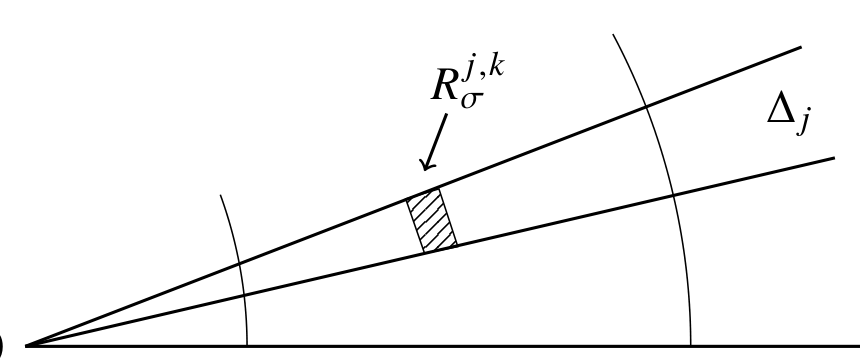
\includegraphics[width=0.5\textwidth]{figs/fig-5-3.png}
\caption{矩形 $R_{\sigma}^{j,k}$.}
\label{fig:5.3}
\end{figure}

此外，假设函数 $\varphi_{\sigma}^{j,k}$ 与 $R_{\sigma}^{j,k}$ 相适应；更精确地,
\begin{align*}
  |D_{v}^{\alpha}\varphi_{\sigma}^{j,k}|\leq
  \begin{cases}
    C_{\alpha}\left(\delta2^{k}\right)^{-\alpha}, & \text{若 } v \text{ 是角平分线方向},\\
    C_{\alpha}\left(\delta^{1/2}2^{k}\right)^{-\alpha}, & \text{若 } v \text{ 垂直于角平分线}.
  \end{cases}
\end{align*}
则
\begin{align*}
  \widehat{S_{t}^{\delta}f}(\xi)=\sum_{k,j,\sigma}\widehat{Q_{k,j,\sigma}^{t}f}(\xi),
\end{align*}
其中
\begin{align*}
  \widehat{Q_{k,j,\sigma}^{t}f}(\xi)=\Theta_{k}(\xi)\phi(|\xi|,t)\psi_{j}(\xi)\varphi_{\sigma}^{j,k}(\xi)\widehat{f}(\xi).
\end{align*}
接着，简化支集的几何: 把 $k$-指标按 $\bmod[|\log_{2}(\delta)|]$ 分成剩余类，使得同一剩余类 $I$ 中、对应不同值 $k_1 > k_2$ 的两个矩形 $R_{\sigma_1}^{j_1,k_1}$ 与 $R_{\sigma_2}^{j_2,k_2}$ 满足: $R_{\sigma_1}^{j_1,k_1}$ 的较小尺寸大于 $2^{k_2}$，即 $2^{k_1}\delta > 2^{k_2}$.

我们还可以假设其他指标 $j$ 与 $\sigma$ 分别取自剩余类 $J$ 与 $\Sigma$（$\bmod 8$）.

于是，除一个允许的因子 $|\log \delta|$ 外，引理将来自估计
\begin{align*}
  \left\|G_{I,J,\Sigma}(f)\right\|_{4}\lesssim\left|\log\delta\right|^{a}\left\|f\right\|_{4}
\end{align*}
对剩余类 $I$，$J$ 与 $\Sigma$ 的任何取法成立，其中
\begin{align*}
  G_{I,J,\Sigma}(f)(x)=\Big(\int_{0}^{\infty}\Big|\sum_{k\in I}\sum_{j\in J}\sum_{\sigma\in\Sigma}Q_{k,j,\sigma}^{t}f(x)\Big|^{2}\frac{\mathrm{d}t}{t}\Big)^{1/2}.
\end{align*}
为简化记号，下面将略去符号 $I, J, \Sigma$，并假设求和指标属于那些固定的剩余类.

有
\begin{align*}
  \left\|G(f)\right\|_{4}^{4}
  =\int_{0}^{\infty}\int_{0}^{\infty}\frac{\mathrm{d}t}{t}\frac{\mathrm{d}u}{u}
  \Big(\int_{\R^{2}}\Big|\sum_{k_{1},j_{1},\sigma_{1}}Q_{k_{1},j_{1},\sigma_{1}}^{t}f(x)
  \sum_{k_{2},j_{2},\sigma_{2}}Q_{k_{2},j_{2},\sigma_{2}}^{u}f(x)\Big|^{2}\mathrm{d}x\Big),
\end{align*}
对内部积分应用 Plancherel 定理，得
\begin{align*}
  \left\|G(f)\right\|_{4}^{4}
  =\int_{0}^{\infty}\int_{0}^{\infty}\frac{\mathrm{d}t}{t}\frac{\mathrm{d}u}{u}
  \Big(\int_{\R^{2}}\Big|\sum_{k_{1},j_{1},\sigma_{1}}\sum_{k_{2},j_{2},\sigma_{2}}
  \Omega_{k_{1},j_{1},\sigma_{1}}^{k_{2},j_{2},\sigma_{2}}(\xi)\Big|^{2}\mathrm{d}\xi\Big),
\end{align*}
其中 $\Omega_{k_{1},j_{1},\sigma_{1}}^{k_{2},j_{2},\sigma_{2}}$ 是
\begin{align*}
  \Theta_{k_{1}}(\xi)\phi(|\xi|,t)\psi_{j_{1}}(\xi)\varphi_{\sigma_{1}}^{j_{1},k_{1}}(\xi)
  \quad\text{与}\quad
  \Theta_{k_{2}}(\xi)\phi(|\xi|,u)\psi_{j_{2}}(\xi)\varphi_{\sigma_{2}}^{j_{2},k_{2}}(\xi)
\end{align*}
的卷积.

现在考虑对 $\Theta_k$，$\psi_j$ 与 $\varphi_\sigma^{j,k}$ 支集所加的条件，得
\begin{align*}
  \|G(f)\|_{4}^{4}\lesssim\int_{\R^{2}}
  \Big(\int_{0}^{\infty}\sum_{k,j,\sigma}\left|Q_{k,j,\sigma}^{t}f(x)\right|^{2}\frac{\mathrm{d}t}{t}\Big)^{2}\mathrm{d}x,
\end{align*}
即只须估计
\begin{align*}
  \Big[\int_{0}^{\infty}\sum_{k,j,\sigma}|Q_{k,j,\sigma}^{t} f(x)|^{2}\frac{\mathrm{d}t}{t}\Big]^{1/2}
\end{align*}
的 $L^{4}$-范数. 为此，首先注意对每组指标 $(k, j, \sigma)$ 与任何函数 $g \in \mathcal{S}(\R^2)$，有逐点不等式
\begin{align*}
  \int_{0}^{\infty}|Q_{k,j,\sigma}^{t}(g)(x)|^{2}\frac{\mathrm{d}t}{t}
  \lesssim\delta\sup_{t}|Q_{k,j,\sigma}^{t}(g)(x)|^{2}.
\end{align*}
这是因为
\begin{align*}
  \{t:Q^{t}_{k,j,\sigma}g(x)\neq 0\}
  &\subset\big\{t:\supp(\widehat{Q^{t}_{k,j,\sigma}g})\ \text{非空}\big\}\\
  &\subset\big\{t:\exists\xi,\ \Theta_{k}(\xi)\phi(|\xi|,t)\varphi^{j,k}_{\sigma}(\xi)\psi_{j}(\xi)\neq 0\big\}=E_{k,j,\sigma},
\end{align*}
而由 $\Theta_{k}$，$\phi$，$\psi_{j}$ 与 $\varphi_{\sigma}^{j,k}$ 的定义，容易得出
\begin{align*}
  \int_{0}^{\infty}E_{k,j,\sigma}(t)\frac{\mathrm{d}t}{t}\lesssim\delta.
\end{align*}
分部积分论证给出核（即 $\Theta_k \phi(|\xi|,t)\varphi_\sigma^{j,k}(\xi)\psi_j(\xi)$ 的傅里叶变换）在离心率 $\delta^{-1/2} = N^{1/2}$ 矩形平均方面的估计，由此得估计
\begin{align*}
  \sup_{t}|Q_{k,j,\sigma}^{t}g(x)|\lesssim M_{\delta^{-1/2}}(\widetilde{Q}_{k,j,\sigma}g)(x),
\end{align*}
其中 $M_{\delta^{-1/2}}$ 表示离心率 $\delta^{-1/2}$ 矩形的 Kakeya 极大函数,
\begin{align*}
  \widehat{\widetilde{Q}_{k,j,\sigma}g}(\xi)=\widetilde{\Theta}_{k}(\xi)\widetilde{\varphi}_{\sigma}^{j,k}(\xi)\widehat{f}(\xi),
\end{align*}
$\widetilde{\Theta}_{k}$ 与 $\widetilde{\varphi}_{\sigma}^{j,k}$ 是分别满足与 $\Theta_{k}$ 和 $\varphi_{\sigma}^{j,k}$ 相同估计、并在其支集上恒等于 $1$ 的适当截断.

于是对每个 $\omega \in L^2(\R^2)$，得
\begin{align*}
  \int_{0}^{\infty}&\int_{\R^{2}}|G f(x)|^{2}\omega(x)\,\mathrm{d}x\,\frac{\mathrm{d}t}{t}
  \lesssim\delta\sum_{j,k,\sigma}\int_{\R^{2}}|\widetilde{Q}_{j,k,\sigma}f(x)|^{2}M_{\delta^{-1/2}}\omega(x)\,\mathrm{d}x\\
  &\leq C_{s}\delta\sum_{\tau=1}^{N^{1/2}}\sum_{k,j}\int_{\R^{2}}
  \left|\widetilde{\widetilde{Q}}_{k,j}^{\tau}f(x)\right|^{2}\left[M(M_{\delta^{-1/2}}\omega)^{s}(x)\right]^{1/s}\mathrm{d}x
\end{align*}
对每个 $s > 1$ 成立，其中
\begin{align*}
  \widehat{\widetilde{Q}}_{k,j}^{\tau}(\xi)=\sum_{\sigma=\tau}^{\tau+N^{1/2}}Q_{k,j,\sigma}(\xi).
\end{align*}
于是对每个 $1 \leq \tau \leq N^{1/2}$，$\widetilde{Q}_{k,j}^{\tau}$ 是适应于边长 $2^k\delta^{1/2}$ 的正方形的截断函数，且集合族 $\{\supp(\widetilde{Q}_{k,j}^{\tau})\}$ 具有与 $\delta$ 无关的有限重叠.

对上述不等式再应用一次引理 5.9，连同 Kakeya 极大函数的已知估计，即可结束证明.
\end{proof}

\section{限制定理}

陈述: 在 $\R^n$（$n > 1$）中，存在指数 $1 \leq p, q \leq \infty$ 与常数 $C(p, q; n) < \infty$，使对每个 Schwartz 类中的 $f$，下列不等式成立:
\begin{align*}
  \Big(\int_{S^{n-1}}|\widehat{f}(\xi)|^{q}\,\mathrm{d}\sigma(\xi)\Big)^{1/q}
  \leq C(p,q;n)\Big(\int_{\R^{n}}|f(x)|^{p}\,\mathrm{d}x\Big)^{1/p}.
\end{align*}
平凡的情形是 $p = 1$，$q = \infty$，但还有其他更有趣的情形.

一旦我们认可这种陈述的可能性，就不难找出允许的 $p$ 与 $q$ 的值.

设 $\varphi$ 是标准 $C^\infty$-bump 函数，使 $\varphi(x) = 1$ 于单位球 $\{|x| \leq 1\}$，在 $\{|x| \leq 2\}$ 之外 $\varphi(x) = 0$.

取 $\delta > 0$，考虑
\begin{align*}
  \varphi_{\delta}(x)=\varphi\Bigl(\frac{x_{1}-1}{\delta},\frac{x_{2}}{\delta^{1/2}},\cdots,\frac{x_{n}}{\delta^{1/2}}\Bigr).
\end{align*}
则
\begin{align*}
  \widehat{\varphi}_{\delta}(\xi)=e^{-2\pi i\xi_{1}}\delta^{(n+1)/2}\widehat{\varphi}(\delta\xi_{1},\delta^{1/2}\xi_{2},\ldots,\delta^{1/2}\xi_{n}).
\end{align*}
设 $\psi_{\delta} = \widehat{\varphi}_{\delta}$. 有
\begin{align*}
  \Big(\int_{S^{n-1}}|\widehat{\psi}_{\delta}(\xi)|^{q}\,\mathrm{d}\sigma(\xi)\Big)^{1/q}\simeq\big(\delta^{(n-1)/2}\big)^{1/q},
\end{align*}
\begin{align*}
  \Big(\int_{\R^{n}}|\psi_{\delta}(x)|^{p}\,\mathrm{d}x\Big)^{1/p}\simeq\delta^{\frac{n+1}{2}[1-1/p]},
\end{align*}
即（$\delta \to 0$）$1/q \geq \frac{n+1}{n-1}[1 - 1/p]$.

考察限制算子的伴随，可以看到限制蕴含: 给定 $g \in L^{q'}(S^{n-1})$，必有
\begin{align*}
  \Big(\int_{\R^{n}}|\widehat{g\,\mathrm{d}\sigma}(x)|^{p'}\,\mathrm{d}x\Big)^{1/p'}
  \lesssim\Big(\int_{S^{n-1}}|g(\xi)|^{q'}\,\mathrm{d}\sigma(\xi)\Big)^{1/q'},
\end{align*}
其中 $1/p + 1/p' = 1$，$1/q + 1/q' = 1$.

于是取 $g \equiv 1$，并利用公式
\begin{align*}
  \widehat{\mathrm{d}\sigma}(x)=c_{n}\frac{J_{(n-2)/2}(2\pi|x|)}{|x|^{(n-2)/2}},
\end{align*}
得到关系 $p'(n-1)/2 > n$，即 $1 \leq p < 2n/(n+1)$.

限制猜想声称，在上述条件下上述陈述成立:
\begin{align*}
  1\leq p<\frac{2n}{n+1},\qquad
  \frac{1}{q}\geq\frac{n+1}{n-1}\Big[1-\frac{1}{p}\Big].
\end{align*}
这是一个引人注目的断言，原因有几条. 首先，傅里叶变换几乎处处有定义，而这里考虑的是它到一个测度为零集合上的限制. 其次，傅里叶变换是线性对象，而 $S^{n-1}$ 高度非线性. 事实上，这是关键: 限制到超平面会归结为一维傅里叶变换在点上的限制，而那无异于对不可积的 $f$ 定义 $\widehat{f}(0) = \int f$. 曲率的作用在这里是本质的，因此把这些结果推广到其他具有非零曲率的曲面是有意义的.

特殊情形 $p = 2$，$q = 2(n+1)/(n+3)$ 众所周知，其证明由 P.~Tomas 与 E.~Stein 用复插值方法获得. 维数 $n = 2$ 的一般情形归功于 C.~Fefferman 与 E.~Stein，但对 $n \geq 3$ 则仍是未知之地，迄今只有部分结果. 下面，我们将呈现二维限制定理的一个``至上主义''证明，见 \cite{b108}.

\begin{theorem}\label{thm:5.19}
若 $f \in L^p(\R^2)$，$1 \leq p < 4/3$，则 $\widehat{f}$ 在 $|\xi| = 1$ 上几乎处处存在，且有
\begin{align*}
  \Big(\int_{|\xi|=1}|\widehat{f}(\xi)|^{q}\,\mathrm{d}\sigma(\xi)\Big)^{1/q}\leq A_{p,q}\left\|f\right\|_{p},
\end{align*}
其中 $q = p'/3 = p/(3(p - 1))$.
\end{theorem}

\begin{proof}
只须证明
\begin{align*}
  \lim_{\delta\rightarrow 0}\left(\delta^{-1}\int_{1-\delta/2\leq|\xi|\leq 1+\delta/2}|\widehat{f}(\xi)|^{q}\,\mathrm{d}\xi\right)^{1/q}
  \leq A_{p,q}\left\|f\right\|_{p}
\end{align*}
在定理的同样条件下成立.

由对偶，只须证明下列估计:
\begin{align*}
  \delta^{-1}\Big\|\sum_{j}a_{j}\widehat{\varphi}_{j}\Big\|_{p'}
  \leq C\Big(\sum_{j}|a_{j}|^{q'}\delta^{1/2}\Big)^{1/q'},
\end{align*}
其中 $p'$ 与 $q'$ 分别是 $p$ 与 $q$ 的共轭指数，$a_j$ 是复数，$\varphi_j$ 是环 $1 - \delta/2 \leq |\xi| \leq 1 + \delta/2$ 的规范分解中``块''（切向 $\delta^{1/2}$，法向 $\delta$）的示性函数. 注意 $p' > 4$. 于是
\begin{align*}
  \Big(\int\Big|\sum_{j,k=1}^{\delta^{-1/2}}a_{j}a_{k}\widehat{\varphi}_{j}\widehat{\varphi}_{k}\Big|^{p'/2}\Big)^{(2/p')\cdot 1/2}
  \leq\Big(\int\Big|\sum_{j,k=1}^{\delta^{-1/2}}a_{j}a_{k}\varphi_{j}*\varphi_{k}\Big|^{r}\Big)^{(1/r)\cdot 1/2},
\end{align*}
其中 $1/r + 2/p = 1$.

由于 $\{\varphi_j * \varphi_k\}$ 的支集``几乎不交''，且 $\mu\{\supp(\varphi_j * \varphi_k)\} \leq \delta^{3/2}(|j - k| + 1)$，得
\begin{align*}
  \|\varphi_{j}*\varphi_{k}\|_{\infty}\leq\frac{\delta^{3/2}}{|j-k|+1}.
\end{align*}
于是有
\begin{align*}
  \Big\|\sum_{j}a_{j}\widehat{\varphi}_{j}\Big\|_{p'}
  \leq C\delta^{\frac{3}{4}(1+1/r)}
  \Big(\sum_{j,k=1}^{\delta^{-1/2}}\frac{|a_{j}|^{r}|a_{k}|^{r}}{(1+|j-k|)^{r-1}}\Big)^{(1/2)\cdot(1/r)}.
\end{align*}
一个分数积分论证给出
\begin{align*}
  \Big\|\sum_{j}a_{j}\widehat{\varphi}_{j}\Big\|_{p'}
  &\leq C\delta^{\frac{3}{4}(1+1/r)}\left[\Big(\sum_{j}|a_{j}|^{2r/(3-r)}\Big)^{3-r}\right]^{1/(2r)}\\
  &\leq C\delta\Big(\sum_{j}|a_{j}|^{q'}\delta^{1/2}\Big)^{1/q'}.
\end{align*}
\end{proof}

注意，这里用到的单位圆的性质只是它的正曲率. 因此，我们实际上证明了一个更一般的定理. 上面给出的``至上主义''证明已被推广到 $\R^3$ 中锥 $\Gamma$ 的情形，其上测度为 $\mathrm{d}\sigma(\xi) = r^{-1}\mathrm{d}\mu(\xi)$，其中 $\mathrm{d}\mu$ 是 $\Gamma$ 上的 Lebesgue 测度，$r$ 是到锥顶点的距离，见 \cite{b97}.

\begin{theorem}\label{thm:5.20}
有先验不等式
\begin{equation}\label{eq:5.4}
  \left(\int_{\Gamma}\left|\widehat{f}(\xi)\right|^{q}\,\mathrm{d}\sigma(\xi)\right)^{1/q}
  \leq C_{p,q}\left\|f\right\|_{p}
\end{equation}
对每个 $f \in \mathcal{S}(\R^3)$ 与 $1 \leq p < 4/3$，$1/q = 3(1 - 1/p)$ 成立.
\end{theorem}

\begin{proof}
由于傅里叶变换对平移与旋转表现良好，不失一般性可设锥的顶点在原点，且由半直线 $z = x$，$z > 0$ 绕 $z$-轴旋转生成. 则有直角坐标方程
\begin{align*}
  z^{2}=x^{2}+y^{2},\qquad z>0,
\end{align*}
可以用
\begin{align*}
  z=r,\qquad x=r\cos\theta,\qquad y=r\sin\theta
\end{align*}
参数化，且在这个参数化下 $\mathrm{d}\sigma = \mathrm{d}r\,\mathrm{d}\theta$.

只须考虑第一象限 $0 \leq \theta \leq \pi/2$，因为锥的对称性使我们能以同样的方式处理其他情形，结果只差一个不同的常数. 把锥分成二进块 $\Gamma_n$，$n \in \Z$，其中 $\Gamma_n$ 是高度 $2^n$ 与 $2^{n+1}$ 两平面之间的锥面部分.

给定 $\delta > 0$，把 $\Gamma_0$ 沿径向膨胀厚度 $\delta r$，得到一个``胖''锥 $\Gamma_0^*$；在高度 $z$（$1 \leq z \leq 2$）处得到环 $0 \leq \theta \leq \pi/2$，$z(1 - \delta/2) \leq r \leq z(1 + \delta/2)$.

\begin{figure}[htbp]
\centering
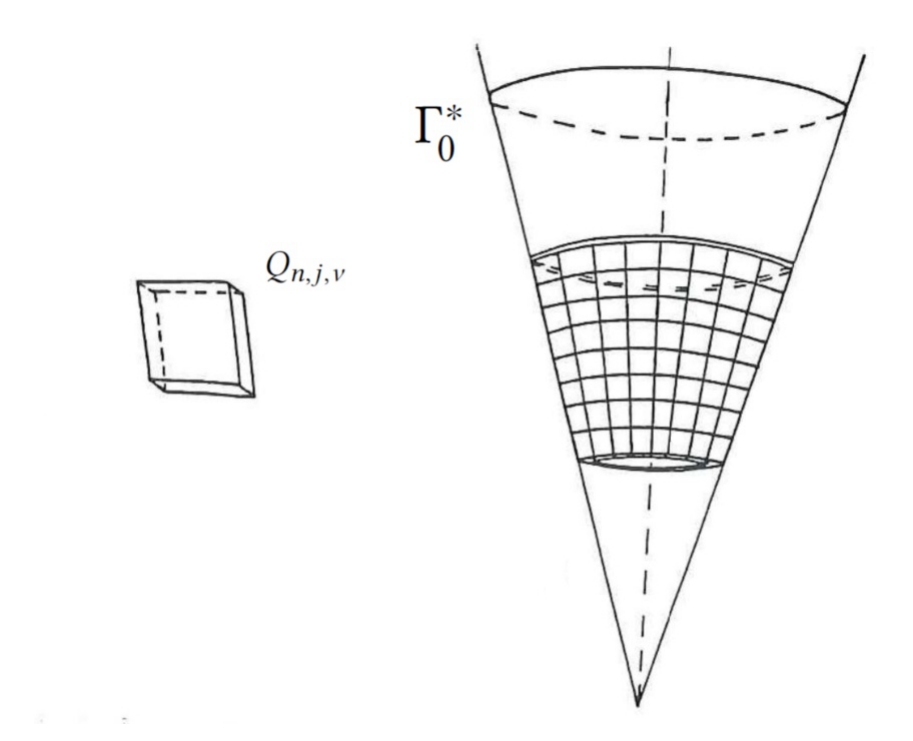
\includegraphics[width=0.42\textwidth]{figs/fig-5-4.png}
\caption{瓦片 $Q_{n,j,\nu}$.}
\label{fig:5.4}
\end{figure}

现在把 $\Gamma_0^*$ 分成 $\delta^{-1/2} \times \delta^{-1/2}$ 个瓦片 $Q_{0,j,\nu}$，其中 $Q_{0,j,\nu}$ 是尺寸 $\delta \times \delta^{1/2} \times \delta^{1/2}$ 的瓦片（板），由 $\Gamma_0^*$ 中高度 $1 + j\delta^{1/2} \leq z \leq 1 + (j+1)\delta^{1/2}$、角方向 $\delta^{1/2}\nu \leq \theta \leq \delta^{1/2}(\nu+1)$ 的点组成.

一旦得到 $\Gamma_0^*$ 的分解，就得到 $\Gamma_n^*$，并由齐性，得到 $\Gamma_n^*$ 到瓦片的类似分解. 这样，$\Gamma_n^*$ 将被分成 $\delta^{-1/2} \times \delta^{-1/2}$ 块 $Q_{n,j,\nu}$，其中 $Q_{n,j,\nu}$ 是尺寸 $2^n \delta \times 2^n \delta^{1/2} \times 2^n \delta^{1/2}$ 的瓦片，位于高度 $2^n + 2^n j \delta^{1/2} \leq z \leq 2^n + 2^n (j+1) \delta^{1/2}$、角方向 $\delta^{1/2}\nu \leq \theta \leq \delta^{1/2}(\nu+1)$. 为便于计算，我们可以假设 $Q_{n,j,\nu}$ 是适应于曲面的矩形瓦片. 见图~\ref{fig:5.4}.

令
\begin{align*}
  \Gamma^{*}=\bigcup_{n}\Gamma_{n}^{*},
\end{align*}
并称 $\varphi_{n,j,\nu}$ 为 $Q_{n,j,\nu}$ 的示性函数.

为证明不等式 \eqref{eq:5.4}，在去奇异化测度的过程中，只须考虑
\begin{align*}
  \lim_{\delta\rightarrow 0}\left(\frac{1}{\delta}\int_{\Gamma^{*}}|\widehat{f}(\xi)|^{q}\frac{\mathrm{d}\xi}{|\xi|^{2}}\right)^{1/q}
  \leq C\left\|f\right\|_{p},
\end{align*}
而为了对偶地证明这个不等式，只须取在每个瓦片上为常数的函数
\begin{align*}
  g(\xi)=\sum_{n,j,\nu}a_{n,j,\nu}\varphi_{n,j,\nu}(\xi),
\end{align*}
使对每个足够小的 $\delta > 0$,
\begin{equation}\label{eq:5.5}
  \Big\|\sum_{n,j,\nu}\frac{a_{n,j,\nu}}{2^{2n/q}}\widehat{\varphi}_{n,j,\nu}\Big\|_{p'}
  \leq C\delta^{1/q}\Big\|\sum_{n,j,\nu}a_{n,j,\nu}\varphi_{n,j,\nu}\Big\|_{q'},
\end{equation}
其中 $p'$ 与 $q'$ 分别是 $p$ 与 $q$ 的对偶指数.

由于只有极限情形 $\delta \to 0$ 有意义，我们考虑锥的任意固定部分 $2^{-M} \leq z \leq 2^M$，并将对固定的 $M$、在 $\delta$ 足够小时以与 $M$ 无关的界证明 \eqref{eq:5.5}.

于是取 $|n| > M$ 时 $a_{n,j,\nu} = 0$. 还取满足
\begin{align*}
  |n-m|\leq|\log_{2}\delta|/2
\end{align*}
的 $\delta$，因为这在几何上意味着（例如若 $m \leq n$）$\Gamma_m^*$ 的直径小于 $\Gamma_n^*$ 中每个瓦片. 这对随后的计算是必要的.

由于 $p' > 4$，可以对 \eqref{eq:5.5} 的左端应用 Hausdorff--Young 定理，其中 $1/s + 2/p' = 1$；则
\begin{align*}
  &\quad\left(\int\Big|\sum_{n,j,\nu}\frac{a_{n,j,\nu}}{2^{2n/q}}\widehat{\varphi}_{n,j,\nu}(\xi)\Big|^{p'}\mathrm{d}\xi\right)^{1/p'}\\
  &=\Big(\int\Big|\sum_{n,m}\sum_{j,k}\sum_{\nu,\mu}\frac{a_{n,j,\nu}a_{m,k,\mu}}{2^{2n/q}2^{2m/q}}
   \widehat{\varphi}_{n,j,\nu}(\xi)\cdot\widehat{\varphi}_{m,k,\mu}(\xi)\Big|^{p'/2}\mathrm{d}\xi\Big)^{(2/p')\cdot 1/2}\\
  &\leq\Big(\int\Big|\sum_{n,m}\sum_{j,k}\sum_{\nu,\mu}\frac{a_{n,j,\nu}a_{m,k,\mu}}{2^{2n/q}2^{2m/q}}
   \varphi_{n,j,\nu}*\varphi_{m,k,\mu}(x)\Big|^{s}\mathrm{d}x\Big)^{1/2s}\\
  &\leq C\Big(\int\Big|\sum_{m\leq n}\sum_{j,k}\sum_{\nu,\mu}\frac{a_{n,j,\nu}a_{m,k,\mu}}{2^{2n/q}2^{2m/q}}
   \varphi_{n,j,\nu}*\varphi_{m,k,\mu}(x)\Big|^{s}\mathrm{d}x\Big)^{1/2s}\\
  &\leq C\Big[\sum_{r=n-m\geq 0}\Big(\int\Big|\sum_{n}\sum_{j,k}\sum_{\nu,\mu}\frac{a_{n,j,\nu}a_{m,k,\mu}}{2^{2n/q}2^{2m/q}}
   \varphi_{n,j,\nu}*\varphi_{m,k,\mu}(x)\Big|^{s}\mathrm{d}x\Big)^{1/s}\Big]^{1/2}\\
  &=\Big[\sum_{r\geq 0}A_{r}\Big]^{1/2},
\end{align*}
其中对固定的 $r \geq 0$，$A_r$ 是上面括号中的表达式，其中一旦取定 $n$，就取 $m = n - r$.

还要注意，因为我们处于锥的固定部分 $2^{-M} \leq z \leq 2^M$，有 $r \leq |\log_2 \delta|/2$.

证明通过仔细分析被积函数中的不同项进行. 为此，需要估计支集的大小以及它们如何重叠.

$z$-坐标的作用体现在竖直重叠，而水平重叠用于研究 $\R^{2}$ 中不同半径圆周上测度 $f(\theta)\,\mathrm{d}\theta$ 的卷积.

为估计 $A_{r}$，如下面的计算所示: 若 $m$ 接近 $n$，则重叠小、尺寸大；但若 $m$ 远离 $n$，则重叠增大、尺寸减小. 妙处在于两者恰好互相补偿.

为度量竖直重叠，若 $m \leq n$，在 $\Gamma_m^*$ 中考虑 $2^m/(\delta^{1/2}2^n)$ 个环 $\Gamma_{m,l}^*$，其中 $\Gamma_{m,l}^*$ 是高度 $\delta^{1/2}2^n$ 的环，由并 $\bigcup_{k,\mu} Q_{m,k,\mu}$ 得到，$\mu$ 取遍所有角方向，$k$ 满足
\begin{align*}
  \delta^{1/2}2^{n}l\leq\delta^{1/2}2^{m}k\leq\delta^{1/2}2^{n}(l+1).
\end{align*}
于是
\begin{align*}
  \left[\Gamma_{m,l}^{*}+\supp(\varphi_{n,j,\nu})\right]
  \cap\left[\Gamma_{m,l'}+\supp(\varphi_{n,j',\nu'})\right]\neq\emptyset
\end{align*}
当 $l + j = l' + j'$ 时成立，而若 $l + j \neq l' + j'$，则此交集具有与 $\delta$ 无关的有限重叠.

由此，固定 $n, m$，$\Gamma_{m,l}^{*}+\supp(\varphi_{n,j,\nu})$ 中的一点至多属于 $2^{m}/(\delta^{1/2}2^{n})$ 个这类和.

由于
\begin{align*}
  \supp\left(\varphi_{n,j,\nu}*\sum_{\mu}\varphi_{m,k,\mu}\right)
  \cap\supp\left(\varphi_{n,j,\nu}*\sum_{\mu}\varphi_{m,k',\mu}\right)\neq\emptyset
\end{align*}
对所有满足 $\supp(\sum_\mu \varphi_{m,k,\mu}) \subset \Gamma_{m,l}^*$ 且 $\supp(\sum_\mu \varphi_{m,k',\mu}) \subset \Gamma_{m,l}^*$ 的 $k, k'$ 成立，而这种指标共有 $2^n/2^m$ 个，于是 $\supp(\varphi_{n,j,\nu} * \sum_\mu \varphi_{m,k,\mu})$ 中的一点至多属于
\begin{align*}
  \left(\frac{2^{m}}{\delta^{1/2}2^{n}}\right)\cdot\left(\frac{2^{n}}{2^{m}}\right)=\delta^{-1/2}
\end{align*}
个这一类的支集.

这就提供了竖直重叠. 于是有
\begin{equation}\label{eq:5.7}
  \begin{aligned}
  \sum_{r}A_{r}
  &=\sum_{\substack{0\leq r\leq\frac{1}{2}|\log_{2}\delta|\\ r=n-m}}
   \left\{\int\left|\sum_{n}\sum_{j,k}\sum_{\nu,\mu}\frac{a_{n,j,\nu}a_{m,k,\mu}}{2^{2n/q}2^{2m/q}}
   \varphi_{n,j,\nu}*\varphi_{m,k,\mu}(x)\right|^{s}\mathrm{d}x\right\}^{1/s}\\
  &\leq C\sum_{\substack{n-m\leq|\log_{2}\delta|\\ m\leq n}}
   \left\{\sum_{n}\sum_{j,k}\frac{\delta^{-(s-1)/2}}{2^{2ns/q}2^{2ms/q}}
   \Big|\Big(\sum_{\nu}a_{n,j,\nu}\varphi_{n,j,\nu}\Big)
   *\Big(\sum_{\mu}a_{m,k,\mu}\varphi_{m,k,\mu}\Big)(x)\Big|^{s}\mathrm{d}x\right\}^{1/s}.
  \end{aligned}
\end{equation}

现在继续估计水平重叠. 必须记住，若两个支集 $Q_{n,j,\nu}$ 与 $Q_{m,k,\mu}$ 的角距离 $|\nu - \mu|$ 很小，则和 $Q_{n,j,\nu} + Q_{m,k,\mu}$ 的尺寸将与 $Q_{n,j,\nu}$ 一样大，且与其他支集会有可观的重叠. 角距离大时则相反.

一旦固定了高度 $j$ 与 $k$，为研究该情形，只须观察它在高度
\begin{align*}
  2^{n}+2^{m}+j\delta^{1/2}2^{n}+k\delta^{1/2}2^{m}
\end{align*}
处垂直于锥轴的截面 $S_{j,k}$ 上的表现，因为 $\supp(\varphi_{n,j,\nu}*\sum_{\mu}\varphi_{m,k,\mu})$ 位于这个高度，而最终的和 $Q_{n,j,\nu}+Q_{m,k,\mu}$ 将由其截面 $S_{j,k}$ 沿 $Q_{n,j,\nu}$ 的竖直方向平移得到.

\begin{figure}[htbp]
\centering
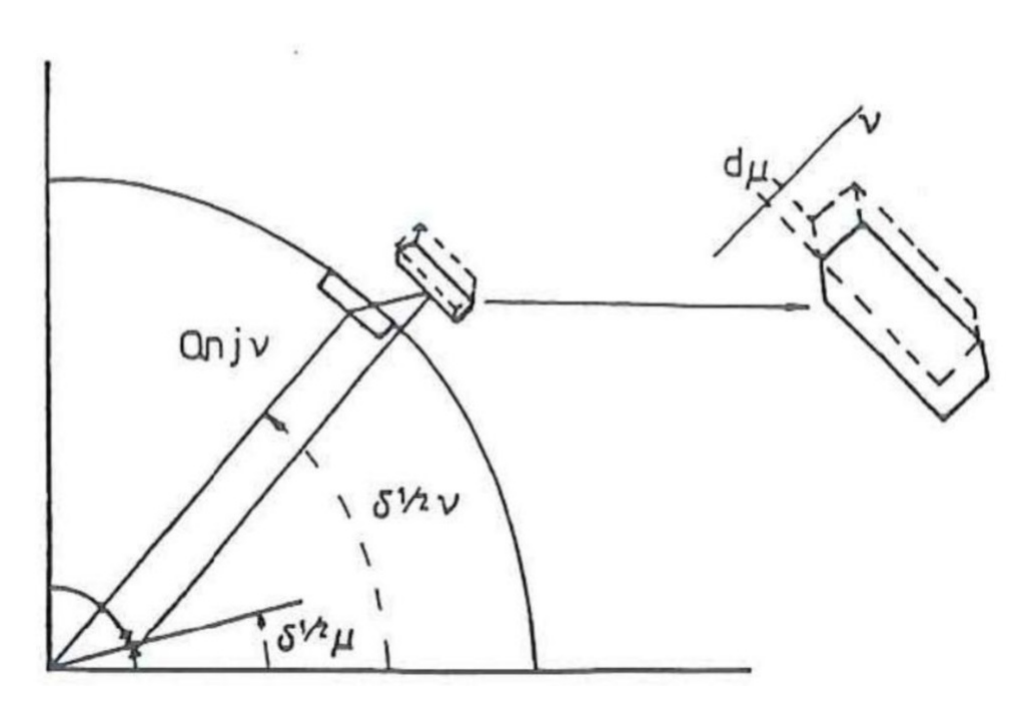
\includegraphics[width=0.52\textwidth]{figs/fig-5-5.png}
\caption{瓦片的和集.}
\label{fig:5.5}
\end{figure}

在 $S_{j,k}$ 平面中，$\supp(\varphi_{n,j,\nu} * \varphi_{m,k,\mu})$ 以点
\begin{align*}
  2^{n}\left(1+\delta^{1/2}j\right)e^{\pi\nu i/2}
  +2^{m}\left(1+\delta^{1/2}k\right)e^{\pi\mu i/2}
\end{align*}
为中心，本质上像一个长 $2^n \delta^{1/2}$、宽
\begin{align*}
  \delta^{1/2}2^{n}+\delta^{1/2}2^{m}\sin\bigl((|\nu-\mu|+1)\delta^{1/2}\bigr)
\end{align*}
的块. 此外，$\supp(\varphi_{n,j,\nu} * \varphi_{m,k,\mu})$ 与 $\supp(\varphi_{n,j,\nu} * \varphi_{m,k,\mu+1})$ 相距平移
\begin{align*}
  \delta^{1/2}2^{m}\sin(|\nu-\mu|\delta^{1/2})\simeq\delta2^{m}|\nu-\mu|,
\end{align*}
这在 $\nu$ 方向上投影即可看出.

为度量卷积 $\varphi_{n,j,\nu} * \varphi_{m,k,\mu}$ 重叠的个数，区分下面两种情形:

情形 (i). $|\nu - \mu| + 1 \leq 2^{n-m}$.

此时，一点至多属于 $N$ 个不同的支集，其中 $N$ 满足
\begin{align*}
  \delta2^{m}|\nu-\mu|+\delta2^{m}(|\nu-\mu|-1)+\cdots+\delta2^{m}(|\nu-\mu|-N)\leq\delta2^{n},
\end{align*}
即 $N \leq 2^{n-m}/(|\nu - \mu| + 1)$.

此外,
\begin{align*}
  |\supp(\varphi_{n,j,\nu}\ast\varphi_{m,k,\mu})|\simeq|\supp(\varphi_{n,j,\nu})|=\delta^{2}2^{3n},
\end{align*}
以及
\begin{align*}
  \|\varphi_{n,j,\nu}\ast\varphi_{m,k,\mu}\|_{\infty}\simeq|\supp(\varphi_{m,k,\mu})|=\delta^{2}2^{3m}.
\end{align*}
因此
\begin{align*}
  \int|\varphi_{n,j,\nu}\ast\varphi_{m,k,\mu}(x)|^{s}\mathrm{d}x
  \leq C\delta^{2s+2}2^{3ms}2^{3n}.
\end{align*}

情形 (ii). $\left|\nu - \mu\right| + 1 \geq 2^{n-m}$.

则当 $\mu$ 变化时 $\supp(\varphi_{n,j,\nu} * \varphi_{m,k,\mu})$ 有有限重叠，且
\begin{align*}
  |\supp(\varphi_{n,j,\nu}*\varphi_{m,k,\mu})|
  &\leq C\delta^{2}2^{2n}2^{m}(|\nu-\mu|+1),\\
  \|\varphi_{n,j,\nu}*\varphi_{m,k,\mu}\|_{\infty}
  &\leq C\delta^{2}2^{n}2^{2m}/(|\nu-\mu|+1).
\end{align*}
于是,
\begin{align*}
  \int\left|\varphi_{n,j,\nu}*\varphi_{m,k,\mu}(x)\right|^{s}\mathrm{d}x
  \leq C\frac{\delta^{2s+2}2^{n(2+s)}2^{m(2s+1)}}{\left(|\nu-\mu|+1\right)^{s-1}}.
\end{align*}

然后，用 (i) 与 (ii) 可以把 \eqref{eq:5.7} 写成
\begin{align*}
  \leq C\sum_{\substack{n-m\leq|\log_{2}\delta|\\ m\leq n}}\Bigg\{&\sum_{n}\sum_{j,k}\frac{\delta^{-(s-1)/2}}{2^{2ns/q}\;2^{2ms/q}}\\
  \times\Big[&\sum_{|\nu-\mu|+1\leq 2^{n-m}}\Big(\frac{2^{n-m}}{|\nu-\mu|+1}\Big)^{s-1}\delta^{2s+2}\;2^{3n}\;2^{3ms}|a_{n,j,\nu}|^{s}|a_{m,k,\mu}|^{s}\\
  &+\sum_{|\nu-\mu|+1\geq 2^{n-m}}\delta^{2s+2}\;2^{n(2+s)}\;2^{m(2s+1)}
   \frac{|a_{n,j,\nu}|^{s}|a_{m,k,\mu}|^{s}}{(|\nu-\mu|+1)^{s-1}}\Big]\Bigg\}^{1/s}\\
  \leq C\sum_{\substack{n-m\leq|\log_{2}\delta|\\ m\leq n}}\Bigg\{\sum_{n}\sum_{j,k}
  &\frac{\delta^{-(s-1)/2}\;\delta^{2s+2}\;2^{m(2s+1)}\;2^{n(2+s)}}{2^{2ns/q}\;2^{2ms/q}}\\
  &\times\sum_{\nu,\mu}\frac{|a_{n,j,\nu}|^{s}|a_{m,k,\mu}|^{s}}{(|\nu-\mu|+1)^{s-1}}\Bigg\}^{1/s},
\end{align*}
再由分数积分论证,
\begin{align*}
  \sum_{\nu,\mu}\frac{\left|a_{n,j,\nu}\right|^{s}\left|a_{m,k,\mu}\right|^{s}}{(|\nu-\mu|+1)^{s-1}}
  \leq C\left(\sum_{\nu}\left|a_{n,j,\nu}\right|^{2s/(3-s)}\right)^{(3-s)/2}
  \left(\sum_{\mu}\left|a_{m,k,\mu}\right|^{2s/(3-s)}\right)^{(3-s)/2}.
\end{align*}
因此，\eqref{eq:5.7} 为
\begin{align*}
  &\leq C\sum_{\substack{n-m\leq|\log_{2}\delta|\\ m\leq n}}
   \delta^{(3s-3)/s}2^{-|n-m|(s-1)/s}\\
  &\quad\cdot\left\{\sum_{n}
   \left(\sum_{j,\nu}|a_{n,j,\nu}|^{2s/(3-s)}\delta^{2}2^{3n}\right)^{(3-s)/2}
   \left(\sum_{k,\mu}|a_{m,k,\mu}|^{2s/(3-s)}\delta^{2}2^{3m}\right)^{(3-s)/2}\right\}^{1/s}\\
  &\leq C\delta^{(3s-3)/s}
   \left(\sum_{\substack{n-m\leq|\log_{2}\delta|\\ m\leq n}}2^{-|n-m|(s-1)/s}\right)
   \left(\sum_{n,j,\nu}|a_{n,j,\nu}|^{2s/(3-s)}\delta^{2}2^{3n}\right)^{(3-s)/s},
\end{align*}
但
\begin{align*}
  \sum_{\substack{n-m\leq|\log_2\delta|\\ m\leq n}}2^{-|n-m|(s-1)/s}\leq C,
\end{align*}
于是我们证明了
\begin{align*}
  \sum_{r\geq 0}A_{r}\leq C\delta^{(3s-3)/s}
  \Big(\sum_{n,j,\nu}|a_{n,j,\nu}|^{2s/(3-s)}\delta^{2}2^{3n}\Big)^{(3-s)/s}.
\end{align*}
现在注意到 $(3s - 3)/2s = 1/q$ 且 $(3 - s)/2s = 1/q'$，最终可以得出
\begin{align*}
  \Big\|\sum_{n,j,\nu}\frac{a_{n,j,\nu}}{2^{2n/q}}\widehat{\varphi}_{n,j,\nu}\Big\|_{p'}
  \leq C\left(\sum_{r}A_{r}\right)^{1/2}
  \leq C\delta^{1/q}\Big\|\sum_{n,j,\nu}a_{n,j,\nu}\varphi_{n,j,\nu}\Big\|_{q'},
\end{align*}
这就是不等式 \eqref{eq:5.5}.
\end{proof}

限制定理已被推广到 $\R^n$ 中曲线的情形（见，例如，\cite{b114,b125}），当 $n \geq 3$ 时对超曲面也有一些部分结果. 但它们的证明，见 \cite{b99,b127,b128}，并不符合本章的``至上主义''观点.

\section{沿平面曲线的希尔伯特变换}

Calderón 与 Zygmund 开创的奇异积分的实变理论已以若干不同方式被推广.

其中一种推广是奇异积分算子
\begin{align*}
  H f(x)=\mathrm{p.v.}\int_{-\infty}^{\infty}f(x-\Gamma(t))\frac{\mathrm{d}t}{t},
\end{align*}
其中 $\Gamma\colon \R \to \R^n$，$n \geq 2$，是过原点的曲线: $\Gamma(0) = 0$. 这个对象——称为沿曲线 $\Gamma$ 的希尔伯特变换——出现在抛物型微分算子的研究以及齐性空间的调和分析中.

这些对象也是傅里叶变换的乘子，因而可以用公式
\begin{align*}
  \widehat{H f}(\xi)=\widehat{f}(\xi)m(\xi)
\end{align*}
定义，其中
\begin{align*}
  m(\xi)=\mathrm{p.v.}\int_{-\infty}^{\infty}\exp(i\xi\cdot\Gamma(t))\frac{\mathrm{d}t}{t}.
\end{align*}
与普通希尔伯特变换的情形（那里 Hardy--Littlewood 极大函数是控制其行为的正算子）类似，可以定义与这些奇异积分相伴的极大算子:
\begin{equation}\label{eq:5.8}
  M f(x)=\sup_{h>0}\frac{1}{2h}\int_{-h}^{h}\left|f(x-\Gamma(t))\right|\mathrm{d}t,
\end{equation}
\begin{equation}\label{eq:5.9}
  H^{*}f(x)=\sup_{\varepsilon>0}\Big|\int_{|t|\geq\varepsilon}f(x-\Gamma(t))\frac{\mathrm{d}t}{t}\Big|.
\end{equation}
人们可能问的第一个自然问题是: 应当对曲线 $\Gamma$ 施加什么条件，才能使 $H$，$H^*$ 与 $M$ 在某个或所有空间 $L^p(\R^n)$ 上有界? 在一系列论文中，A.~Nagel，E.~Stein，S.~Wainger 等人 \cite{b120,b121} 获得了涉及 $\Gamma$ 曲率某种``正性''的结果，利用了它所蕴含的乘子 $m(\xi)$ 的衰减. 证明由复插值方法的巧妙运用，连同涉及某些平方函数的 Tauber 型论证完成. 在 \cite{b121} 中观察到，对 $\R^2$ 中凸曲线 $\Gamma(t) = (t, \gamma(t))$（$\gamma(0) = \gamma'(0) = 0$），存在 $H$ 在 $L^2(\R^2)$ 有界的充要条件: 当 $\gamma$ 为偶函数（相应地，奇函数）时，条件是 $\gamma'(t)$（相应地，$h(t) = t\gamma'(t) - \gamma(t)$）必须具有倍时性质，即对某个固定常数 $C$ 与每个 $t > 0$，$\gamma'(Ct) \geq 2\gamma'(t)$（相应地，$h(Ct) \geq 2h(t)$）. $L^p$-估计的范围在 \cite{b111} 中从 $L^2$ 推广到 $L^p$，$4/3 < p < 4$.

考虑 $\R^2$ 中的 $C^1$ 曲线 $\Gamma = \{(t, \gamma(t)): -\infty < t < +\infty\}$，$\gamma(0) = \gamma'(0) = 0$，具有如下性质:

(a) $\gamma$ 是双凸的，即 $|\gamma'(t)|$ 在 $(-\infty, 0)$ 上递减，在 $(0, +\infty)$ 上递增.

(b) $\gamma$ 具有倍时性，即存在常数 $C > 1$，使 $|\gamma'(Ct)| \geq 2|\gamma'(t)|$.

(c) $\gamma$ 是平衡的，意思如下: 存在 $k > 1$，使对每个 $t > 0$ 有 $|\gamma(k^{-1}t)| \leq |\gamma(-t)| \leq |\gamma(kt)|$.

\begin{theorem}\label{thm:5.21}
在关于曲线的假设 (a)，(b) 与 (c) 之下，奇异积分 $H$ 与极大函数 $M$ 和 $H^*$ 是 $L^p(\R^2)$ 上的有界算子，对每个 $p$，$1<p<\infty$ 成立.
\end{theorem}

$M$ 与 $H^{*}$ 有界性的直接推论是:

\begin{corollary}\label{cor:5.22}
对每个 $f \in L^p(\R^2)$，$1 < p < \infty$,
\begin{align*}
  &\lim_{\varepsilon\rightarrow 0}\frac{1}{2\varepsilon}\int_{-\varepsilon}^{\varepsilon}f(x-\Gamma(t))\,\mathrm{d}t=f(x)\quad\text{a.e.},\\
  &\lim_{\varepsilon\rightarrow 0}\int_{|t|>\varepsilon}f(x-\Gamma(t))\frac{\mathrm{d}t}{t}=H f(x)\quad\text{a.e.}
\end{align*}
\end{corollary}

定理 5.21 对平面凸曲线沿曲线的希尔伯特变换的性质给出了相当完整的分析. 对每个固定的 $p$，$1 < p < \infty$，若曲线为偶，则倍时性质是 $L^p$-有界性的充要条件. 同样，对双凸曲线，平衡条件对 $H$ 的 $L^2$-有界性是必要的，正如后面 5.7.5 节所证明的. 对这样的曲线，不能只获得 $L^p(\R^2)$ 中某些 $p$ 的希尔伯特变换有界性而不获得全范围 $1 < p < \infty$；这反过来解释了该理论的成功，与球面求和乘子分析中的情形形成对照.

\subsection{算子的分解与证明梗概}

所有 $L^p$ 估计都将对 $f \in \mathcal{S}(\R^2)$ 证明，再由连续性扩张. 定义奇异测度 $M_k$ 与 $h_k$（$k \in \Z$），使
\begin{align*}
  \widehat{M}_{k}(\xi,\eta)=\int_{1\leq|t|\leq 2}\exp\left\{i(2^{k}t\xi+\gamma(2^{k}t)\eta)\right\}\mathrm{d}t,
\end{align*}
\begin{align*}
  \widehat{h}_{k}(\xi,\eta)=\int_{1\leq|t|\leq 2}\exp\left\{i(2^{k}t\xi+\gamma(2^{k}t)\eta)\right\}\frac{\mathrm{d}t}{t},
\end{align*}
并考虑我们的算子的下列基本分解:
\begin{equation}\label{eq:5.10}
  Mf(x)\simeq\sup_{k}|M_{k}*f(x)|,
\end{equation}
\begin{equation}\label{eq:5.11}
  H f(x)=\sum_{k=-\infty}^{\infty}h_{k}*f(x),
\end{equation}
\begin{equation}\label{eq:5.12}
  H^{*}f(x)\simeq\sup_{k}\Big|\sum_{n>k}h_{n}*f(x)\Big|.
\end{equation}
我们还将使用下列平方函数:
\begin{equation}\label{eq:5.13}
  G f(x)=\Big(\sum_{k=-\infty}^{\infty}|\widetilde{M}_{k}f(x)|^{2}\Big)^{1/2},
\end{equation}
其中
\begin{align*}
  \widehat{\widetilde{M}_{k}f}(\xi,\eta)=\left[\widehat{M}_{k}(\xi,\eta)-\widehat{\Phi}(2^{k}\xi)\widehat{M}_{k}(0,\eta)\right]\widehat{f}(\xi,\eta),
\end{align*}
$\Phi$ 是 Schwartz 类中满足 $\Phi(0) = 1$ 的适当函数.

极大函数 $Mf$ 的有界性证明基于如下策略: 有逐点控制 $M f(x) \leq G f(x) + f^*(x)$，其中 $f^*$ 表示 $f$ 的强极大函数. 首先用 Plancherel 定理证明 $Gf$ 的 $L^2$-有界性. 这蕴含 $Mf$ 的同样结果，再由如今众所周知的基于向量值不等式与频率空间特殊 Littlewood--Paley 分解的论证，蕴含平方函数 $Gf$ 的 $L^p$ 估计（$4/3 < p < 4$）. 一般地，$M$ 的 $L^p$ 估计蕴含 $G$ 的 $L^q$ 估计，其中 $|1/q - 1/2| < 1/(2p)$；因此，bootstrap 论证将给出整个 $1 < p < \infty$ 的范围.

曲线的倍时条件将用于定义角 Littlewood--Paley 分解. 为简单起见，假设倍时常数为 $C = 2$. 于是考虑角区域
\begin{align*}
  \Delta_{k}^{\pm}=\Big\{(\xi,\eta):
  \frac{1}{2}|\gamma^{\prime}(\pm 2^{k})|<\frac{|\xi|}{|\eta|}<2|\gamma^{\prime}(\pm 2^{k+1})|\Big\},\qquad k\in\Z.
\end{align*}
结果表明 $\{\Delta_k^+\}_{-\infty}^{\infty}$ 是 $\R^2$ 的缺项分解，具有有限重叠: 若 $|k - h| \geq 3$ 则 $\Delta_h^+ \cap \Delta_k^+ = \emptyset$，对 $\{\Delta_k^-\}$ 亦然.

\subsection{极大算子与平方函数}

设 $\Delta_{k} = \Delta_{k}^{+} \cup \Delta_{k}^{-}$，定义投影算子 $T_{k}$:
\begin{align*}
  \widehat{(T_{k}f)}=\widehat{f}\chi_{\Delta_{k}},\qquad k\in\Z.
\end{align*}

\begin{lemma}\label{lem:5.23}
对每个 $p$，$1 < p < \infty$，有
\begin{equation}\label{eq:5.14}
  \left\|\Big(\sum_{k}\left|T_{k}f\right|^{2}\Big)^{1/2}\right\|_{p}\leq c_{p}\left\|f\right\|_{p},
\end{equation}
\begin{equation}\label{eq:5.15}
  \Big\|\sum_{k}T_{k}f_{k}\Big\|_{p}\leq c_{p}\Big\|\Big(\sum_{k}|f_{k}|^{2}\Big)^{1/2}\Big\|_{p},
\end{equation}
\begin{equation}\label{eq:5.16}
  \left\|\sup_{k}\left|\sum_{n\geq k}T_{n}f\right|\right\|_{p}\leq c_{p}\left\|f\right\|_{p}.
\end{equation}
\end{lemma}

不等式 \eqref{eq:5.14} 如今众所周知（参考文献见 \cite{b98}），\eqref{eq:5.15} 是其对偶形式；\eqref{eq:5.16} 由 \eqref{eq:5.14} 按证明傅里叶级数缺项收敛的同样方式得出.

\begin{lemma}\label{lem:5.24}
算子
\begin{align*}
  \Gamma f(x)=\sup_{h>0}\frac{1}{2h}\int_{-h}^{h}\left|f(x-\gamma(t))\right|\mathrm{d}t
\end{align*}
是 $L^p(\R)$（$1 < p < \infty$）上的有界算子.
\end{lemma}

证明由于 $\gamma'$ 的单调性是显然的:
\begin{align*}
  \frac{1}{h}\int_{0}^{h}f(x-\gamma(t))\,\mathrm{d}t
  &=\frac{1}{h}\int_{0}^{\gamma(h)}f(x-u)\frac{\mathrm{d}u}{\gamma'(\gamma^{-1}(u))}\\
  &=\int_{0}^{c}f(x-u)\varphi(u)\,\mathrm{d}u\leq f^{*}(x),
\end{align*}
（Hardy--Littlewood 极大函数），因为 $\varphi(u)$ 非负、递减且满足 $\int_{0}^{c}\varphi(u)\,\mathrm{d}u = 1$. 对区间 $[-h, 0]$ 上的平均，同样的论证成立.

\begin{lemma}\label{lem:5.25}
设 $\Phi \in \mathcal{S}(\R)$ 满足 $\chi_{[-1,1]} \leq \Phi \leq \chi_{[-2,2]}$. 则
\begin{align*}
  \left|\widehat{M}_{k}(\xi,\eta)-\widehat{\Phi}(2^{k}\xi)\widehat{M}_{k}(0,\eta)\right|
  \leq C\min\bigl(2^{k}|\xi|,(2^{k}|\xi|)^{-1}\bigr),
\end{align*}
对所有 $(\xi,\eta)\notin\Delta_{k}$ 成立. 对 $\widehat{h}_{k}(\xi,\eta)$ 代替 $\widehat{M}_{k}(\xi,\eta)$，同样的估计成立.
\end{lemma}

\begin{proof}
$2^k|\xi| \leq 1$ 情形的估计是平凡的，因为 $M_k$ 是支于 $\{(x_1, x_2) : |x_1| \leq 2^{k+1}\}$ 的测度. 对 $2^k|\xi| > 1$，用 van der Corput 引理:
\begin{align*}
  \widehat{M}_{k}(\xi,\eta)=\int_{1}^{2}e^{i g_{k}(t)}\,\mathrm{d}t+\int_{1}^{2}e^{i l_{k}(t)}\,\mathrm{d}t,
\end{align*}
其中
\begin{align*}
  |g_{k}^{\prime}(t)|=|2^{k}(\xi+\gamma^{\prime}(2^{k}t)\eta)|,\qquad
  |l_{k}^{\prime}(t)|=|2^{k}(\xi+\gamma^{\prime}(-2^{k}t)\eta)|.
\end{align*}
若 $|\xi| \geq 2|\eta|\cdot|\gamma'(2^{k+1})|$，则 $|g_k'(t)| \geq 2^{k-1}|\xi|$. 若 $|\xi| \leq \frac{1}{2}|\eta|\cdot|\gamma'(2^k)|$，则也有 $|g_k'(t)| \geq 2^{k-1}|\gamma'(2^k t)|\cdot|\eta| \geq 2^k|\xi|$；对 $l'_k$ 情形类似. 最后，这四种情形的补集正对应点 $(\xi, \eta) \in \Delta_k$. 对 $\widehat{h}_k(\xi, \eta)$ 的证明本质相同.
\end{proof}

假设 $U_k f = U_k * f$ 是在 $L^\infty(\R^n)$ 上一致有界的正算子序列，考虑 $U^* f(x) = \sup_k |U_k * f(x)|$.

\begin{lemma}\label{lem:5.26}
若 $U^* f(x) = \sup_k |U_k * f(x)|$ 在 $L^q(\R^n)$ 上有界，则
\begin{align*}
  \left\|\Big(\sum_{k}|U_{k}f_{k}|^{2}\Big)^{1/2}\right\|_{p}
  \leq c_{p}\left\|\Big(\sum_{k}|f_{k}|^{2}\Big)^{1/2}\right\|_{p}
\end{align*}
对 $|1/p - 1/2| = 1/(2q)$ 成立.
\end{lemma}

这是众所周知的结果，在这里陈述只是为了厘清定理 5.21 证明的表述. 极大函数估计的证明依赖于下面这个条件性质的命题.

\begin{lemma}\label{lem:5.27}
假设对某个 $q$ 有 $\|Mf\|_q \leq C\|f\|_q$. 则对所有满足 $|1/p - 1/2| < 1/(2q)$ 的 $p$，有不等式
\begin{align*}
  \left\|G f\right\|_{p}\leq C_{p}\left\|f\right\|_{p},
\end{align*}
其中 $G$ 由 \eqref{eq:5.13} 定义.
\end{lemma}

\begin{proof}
回忆 $T_{k}f = \chi_{\Delta_{k}}\cdot\widehat{f}$，写
\begin{align*}
  f^{k}=f-T_{k}f,
\end{align*}
以及
\begin{align*}
  S_{k}f=\widehat{f}\cdot\chi\{(\xi,\eta):2^{k}\leq|\xi|\leq 2^{k+1}\}.
\end{align*}
则
\begin{align*}
  G f\leq\Big(\sum_{k}|\widetilde{M}_{k}*T_{k}f|^{2}\Big)^{1/2}
  +\Big(\sum_{k}|\widetilde{M}_{k}*f^{k}|^{2}\Big)^{1/2}=\mathbf{I}+\mathbf{II}.
\end{align*}
现在注意，由假设与引理 5.24，$\sup_k(|\widetilde{M}_k|*f)$ 是 $L^q$ 上的有界算子. 因此
\begin{align*}
  \left\|\mathrm{I}\right\|_{p}\leq C_{p}\left\|\Big(\sum_{k}\left|T_{k}f\right|^{2}\Big)^{1/2}\right\|_{p}\leq C_{p}\left\|f\right\|_{p}
\end{align*}
由引理 5.26 与引理 5.23.

有
\begin{align*}
  \mathrm{II}=\Big(\sum_{k}\Big|\widetilde{M}_{k}*\Big(\sum_{j=-\infty}^{\infty}S_{j+k}f^{k}\Big)\Big|^{2}\Big)^{1/2}
  \leq\sum_{j}\Big(\sum_{k}|\widetilde{M}_{k}*S_{j+k}f^{k}|^{2}\Big)^{1/2}
  =\sum_{j}\mathrm{II}_{j}.
\end{align*}
我们将证明:
\begin{align*}
  \left\|\mathrm{II}_{j}\right\|_{2}\leq C2^{-\left|j\right|}\left\|f\right\|_{2},
  \qquad
  \left\|\mathrm{II}_{j}\right\|_{p_{0}}\leq C\left\|f\right\|_{p_{0}},
  \quad \left|\frac{1}{2}-\frac{1}{p_{0}}\right|=\frac{1}{2q}.
\end{align*}
插值，将得到
\begin{align*}
  \left\|\mathrm{II}\right\|_{p}\leq\sum_{j}\left\|\mathrm{II}_{j}\right\|_{p}
  \leq\sum_{j}C2^{-\theta\left|j\right|}\left\|f\right\|_{p}
  \leq C_{p}\left\|f\right\|_{p},
  \qquad \frac{1}{p}=\frac{1-\theta}{p_{0}}+\frac{\theta}{2}.
\end{align*}
对 $L^{2}$-不等式用 Plancherel 定理:
\begin{align*}
  \|\mathrm{II}_{j}\|_{2}^{2}
  &=\sum_{k}\int_{\substack{|\xi|\sim 2^{-j-k}\\ (\xi,\eta)\notin\Delta_{k}}}
   |\widehat{M}_{k}(\xi,\eta)-\widehat{\Phi}(2^{k}\xi)\widehat{M}_{k}(0,\eta)|^{2}|\widehat{f}(\xi,\eta)|^{2}\,\mathrm{d}\xi\,\mathrm{d}\eta\\
  &\stackrel{(\text{由引理~5.25})}{\leq}C\int|\widehat{f}(\xi,\eta)|^{2}(2^{-|j|})^{2}\,\mathrm{d}\xi\,\mathrm{d}\eta
  =C2^{-2|j|}\|f\|_{2}^{2}.
\end{align*}
最后,
\begin{align*}
  \|\mathrm{II}_{j}\|_{p_{0}}
  &\leq C_{p_{0}}\left\|\Big(\sum_{k}|S_{j+k}f^{k}|^{2}\Big)^{1/2}\right\|_{p_{0}}\\
  &\leq C_{p_{0}}\left\{\left\|\Big(\sum_{k}|S_{j+k}f|^{2}\Big)^{1/2}\right\|_{p_{0}}
   +\left\|\Big(\sum_{k}|S_{j+k}(T_{k} f)|^{2}\Big)^{1/2}\right\|_{p_{0}}\right\}\\
  &\leq C_{p_{0}}\left\{\|f\|_{p_{0}}+\left\|\Big(\sum_{k}|T_{k} f|^{2}\Big)^{1/2}\right\|_{p_{0}}\right\}
  \leq C_{p_{0}}\|f\|_{p_{0}}.
\end{align*}
\end{proof}

为完成极大算子定理的证明，使用控制
\begin{align*}
  Mf(x)\leq 2\sup_{k}|M_{k}*f(x)|
  \leq 2\sup_{k}|\widetilde{M}_{k}*f(x)|+2Nf(x)
  \leq 2Gf(x)+2Nf(x),
\end{align*}
其中 $N$ 是 $x_1$-变量的 Hardy--Littlewood 算子与 $x_2$-变量引理 5.24 的算子 $\Gamma$ 的复合. 现在可以应用 5.7.1 节勾画的 bootstrap 论证，给出对 $1 < p \leq \infty$ 的 $\|M f\|_p \leq C_p \|f\|_p$.

\subsection{奇异积分}

$Hf$ 的估计将基于与引理 5.27 类似的论证，连同算子 $h_k * f$ 被极大算子 $Mf$ 控制这一事实.

首先考虑 $\gamma(t)$ 为偶函数的情形，使 $\widehat{h}_{k}(0,\eta)=0$. 所用记号与引理 5.27 相同:
\begin{align*}
  H f=\sum_{k}h_{k}*T_{k}f+\sum_{k}h_{k}*f^{k}=H_{\mathrm{I}}f+H_{\mathrm{II}}f.
\end{align*}
利用引理 5.23 与 5.26，以及 $\sup_k |h_k| * f \leq M f$ 的事实，得到
\begin{align*}
  \left\|H_{\mathrm{I}}f\right\|_{p}
  &=\left\|\sum_{k}T_{k}(h_{k}*T_{k}f)\right\|_{p}
  \leq C_{p}\left\|\Big(\sum_{k}|h_{k}*T_{k}f|^{2}\Big)^{1/2}\right\|_{p}\\
  &\leq C_{p}\left\|\Big(\sum_{k}|T_{k}f|^{2}\Big)^{1/2}\right\|_{p}
  \leq C_{p}\left\|f\right\|_{p}.
\end{align*}
另一方面,
\begin{align*}
  |H_{\mathrm{II}}f|=\Big|\sum_{k}h_{k}*\sum_{j=-\infty}^{\infty}S_{j+k}f^{k}\Big|
  \leq\sum_{j}\Big|\sum_{k}h_{k}*S_{j+k}f^{k}\Big|
  =\sum_{j}|\mathrm{II}_{j}|.
\end{align*}
由于 $h_{k}(0,\eta)=0$，引理 5.25 与 Plancherel 定理给出
\begin{align*}
  \|\mathrm{II}_{j}\|_{2}^{2}
  &=\sum_{k}\int_{\substack{|\xi|\sim 2^{-j-k}\\ (\xi,\eta)\notin\Delta_{k}}}
   |\widehat{f}(\xi,\eta)|^{2}|\widehat{h}_{k}(\xi,\eta)|^{2}\,\mathrm{d}\xi\,\mathrm{d}\eta
  \leq C\int|\widehat{f}(\xi,\eta)|^{2}2^{-2|j|}\,\mathrm{d}\xi\,\mathrm{d}\eta\\
  &\leq C2^{-2|j|}\|f\|_{2}^{2}.
\end{align*}
在 $L^{p}$（$1 < p < \infty$）中有一致估计
\begin{align*}
  \|\mathrm{II}_{j}\|_{p}
  &=\Big\|\sum_{k}S_{j+k}(h_{k}*S_{j+k}f^{k})\Big\|_{p}
  \leq C_{p}\left\|\Big(\sum_{k}|h_{k}*(S_{j+k}f^{k})|^{2}\Big)^{1/2}\right\|_{p}\\
  &\leq C_{p}\left\|\Big(\sum_{k}|S_{j+k}f^{k}|^{2}\Big)^{1/2}\right\|_{p}
  \leq C_{p}\|f\|_{p},
\end{align*}
证明以插值和求等比级数结束.

对一般曲线的情形，分解
\begin{align*}
  h_{k}=\widetilde{h}_{k}+m_{k},
\end{align*}
其中，$\Phi$ 如前,
\begin{align*}
  \widehat{m}_{k}(\xi,\eta)=\widehat{\Phi}(2^{k}\xi)\cdot\widehat{h}_{k}(0,\eta).
\end{align*}
则 $h_{k}$ 的傅里叶变换满足与偶曲线情形相同的估计，即
\begin{align*}
  |\widehat{h}_{k}(\xi,\eta)|\leq C\min(2^{k}|\xi|,(2^{k}|\xi|)^{-1}),\qquad (\xi,\eta)\notin\Delta_{k},
\end{align*}
且 $\sup_k |\widetilde{h}_k| * f \leq M f + N f$ 对所有 $p > 1$ 在 $L^p(\R^2)$ 上有界. 于是，前面的论证给出
\begin{align*}
  \left\|\sum_{k}\widetilde{h}_{k}*f\right\|_{p}\leq C_{p}\left\|f\right\|_{p},\qquad 1<p<\infty.
\end{align*}
接下来需要估计 $h_k(0, \eta)$ 的衰减. 正是在这里，曲线平衡的假设发挥作用. 为简单起见，假设平衡常数 $k \leq 2$. 定义 $\lambda_k = |\gamma(2^k)|$，$k \in \Z$，使 $\{\lambda_k\}_{k \in \Z}$（由凸性）是缺项序列，而平衡条件蕴含 $\lambda_{k-1} \leq |\gamma(-2^k)| \leq \lambda_{k+1}$，$k \in \Z$. 现在，对小 $\eta$，有
\begin{align*}
  |\widehat{h}_{k}(0,\eta)|
  &=\Big|\int_{1\leq|t|\leq 2}[e^{i\eta\gamma(2^{k} t)}-1]\frac{\mathrm{d}t}{t}\Big|
  \leq(\log 2)\;|\eta|\;(\left|\gamma(2^{k+1})\right|+\left|\gamma(-2^{k+1})\right|)\\
  &\leq C\cdot\lambda_{k+2}\cdot|\eta|.
\end{align*}
对大 $\eta$，再次用 van der Corput 引理. 由于
\begin{align*}
  \left|\frac{\mathrm{d}}{\mathrm{d}t}(\eta\gamma(2^{k} t))\right|
  =|2^{k}\eta\gamma^{\prime}(2^{k} t)|\geq\lambda_{k-1}|\eta|,\qquad 1\leq|t|\leq 2,
\end{align*}
得到
\begin{align*}
  |\widehat{h}_{k}(0,\eta)|\leq C\left(\lambda_{k-1}|\eta|\right)^{-1}.
\end{align*}
现在把偶情形的同样论证用于以 $\tilde{S}_{j}$ 代替 $S_{j}$，其中
\begin{align*}
  \widehat{\widetilde{S}_{j}f}(\xi,\eta)=\widehat{f}(\xi,\eta)\cdot\chi_{I_{j}}(\eta),
\end{align*}
$I_{j}=[\lambda_{j+1}^{-1},\lambda_{j}^{-1}]\cup[-\lambda_{j}^{-1},-\lambda_{j+1}^{-1}]$. 则
\begin{align*}
  \sum_{k}m_{k}*f=\sum_{j,k}m_{k}*\tilde{S}_{j+k}f=\sum_{j=-\infty}^{\infty}A_{j}f.
\end{align*}
一致估计 $\|A_j f\|_p \leq C_p \|f\|_p$（$1 < p < \infty$）如偶情形一样得出. 在 $L^2$ 中，有
\begin{align*}
  \|A_{j}f\|_{2}^{2}
  =\sum_{k}\int_{\R}\int_{I_{j+k}}|\widehat{f}(\xi,\eta)|^{2}|m_{k}(\xi,\eta)|^{2}\,\mathrm{d}\xi\,\mathrm{d}\eta.
\end{align*}
若 $j > 1$ 且 $\eta \in I_{j+k}$，则
\begin{align*}
  |m_{k}(\xi,\eta)|\leq\frac{\lambda_{k+2}}{\lambda_{k+j}}\leq\rho^{2-j},
\end{align*}
其中 $\rho > 1$ 是序列 $\{\lambda_k\}_{k \in \Z}$ 的缺项常数. 当 $j < -1$ 且 $\eta \in I_{j+k}$ 时,
\begin{align*}
  |m_{k}(\xi,\eta)|\leq\frac{\lambda_{j+k+1}}{\lambda_{k-1}}\leq\rho^{2+j}.
\end{align*}
于是,
\begin{align*}
  \|A_{j}f\|_{2}\leq C\rho^{-|j|}\|f\|_{2},\qquad -\infty<j<\infty,
\end{align*}
证明到此结束.

\subsection{极大希尔伯特变换}

这里将证明算子 $H^{*}f(x)$（由 \eqref{eq:5.12} 定义）对所有 $1 < p < \infty$ 的 $L^{p}$-有界性. 由于
\begin{align*}
  H^{*}f(x)\leq M f(x)+\sup_{k}\Big|\sum_{n\geq k}h_{n}*f(x)\Big|,
\end{align*}
只须考虑极大算子:
\begin{align*}
  \sup_{k}\left|\sum_{n\geq k}h_{n}*f\right|.
\end{align*}
为简单起见，只在偶曲线的情形做这件事；处理一般平衡曲线所需的修改本质包含在 5.7.3 节最后的计算中. 定义 $\Phi \in \mathcal{S}(\R)$ 如引理 5.25，写 $\widehat{\Phi}_k(\xi) = \widehat{\Phi}(2^k\xi)$，并用 $*^{(1)}$ 表示第一个变量上的卷积. 然后如下分解截断的希尔伯特变换:
\begin{align*}
  &\sum_{n\geq k}h_{n}*f\\
  &=\Phi_{k}*^{(1)}\left\{H f-\sum_{n<k}h_{n}*f\right\}
   +\left(\delta-\Phi_{k}\right)*^{(1)}\sum_{n\geq k}h_{n}*T_{n}f
   +\left(\delta-\Phi_{k}\right)*^{(1)}\sum_{n\geq k}h_{n}*f^{n}\\
  &=A_{k}f+B_{k}f+C_{k}f,
\end{align*}
并且需要估计 $\sup_k |A_{k}f|$，$\sup_k |B_{k}f|$ 与 $\sup_k |C_{k}f|$. 在此过程中，将使用下列极大算子:

(a) $g_{1}^{*}(x)$: $g(x_{1}, x_{2})$ 在 $x_{1}$-方向上的 Hardy--Littlewood 极大函数.

(b) $Ng(x)$: 作用于 $x_1$ 变量的 Hardy--Littlewood 极大算子，以及引理 5.24 中作用于 $x_2$ 的算子 $\Gamma$（该算子出现在 5.7.2 节末尾）.

(c) $T^*g(x) = \sup_k |T_k g(x)|$.

(d) $S^* g(x) = \sup_k |\sum_{n \geq k} T_n g(x)|$（见引理 5.23）.

(e) $Mf(x)$: 沿曲线 $\Gamma$ 的极大算子.

所有这些都在每个 $1 < p < \infty$ 的 $L^p(\R^2)$ 上有界. 现在，为估计 $A_k f$，首先注意核 $\Phi_k *^{(1)} \sum_{n<k} h_n$ 的作用逐点地被极大算子 $N$ 的作用控制. 只须在点 $x = 0$、$k = 0$ 处证明；给定测试函数 $g$，有
\begin{align*}
  \left|\left\langle\Phi_{*}*^{(1)}\sum_{n<0}h_{n},g\right\rangle\right|
  &=\left|\int_{-\infty}^{\infty}\left\{\mathrm{p.v.}\int_{-1}^{1}g\left(s+t,\gamma(t)\right)\frac{\mathrm{d}t}{t}\right\}\Phi(s)\,\mathrm{d}s\right|\\
  &=\left|\int_{-\infty}^{\infty}\int_{-1}^{1}\left[\Phi(s-t)-\Phi(s)\right]g\left(s,\gamma(t)\right)\frac{\mathrm{d}t}{t}\,\mathrm{d}s\right|\\
  &\leq C\int_{-1}^{1}\int_{-\infty}^{\infty}\frac{1}{1+s^{2}}\left|g\left(s,\gamma(t)\right)\right|\mathrm{d}s\,\mathrm{d}t
  \leq Ng(0)
\end{align*}
（第二个等式用到了 $\gamma$ 为偶函数的事实）. 因此,
\begin{align*}
  \sup_{k}\left|A_{k}f(x)\right|\leq C\left[(H f)_{1}^{*}(x)+N f(x)\right].
\end{align*}
对第二项，由于 $\{T_n\}_{n\in\Z}$ 是正交投影，可以写 $h_n*T_nf = T_n(\sum_j h_j*T_j f)$. 回忆 5.7.4 节中 $Hf$ 被分解为 $Hf = H_{\mathrm{I}}f + H_{\mathrm{II}}f$，且两部分对所有 $1 < p < \infty$ 都在 $L^p$ 上有界. 于是,
\begin{align*}
  \sup_{k}\left|B_{k}f(x)\right|
  =\sup_{k}\left|\left(\delta-\Phi_{k}\right)*^{(1)}\sum_{n\geq k}T_{n}(H_{\mathrm{I}}f)(x)\right|
  \leq C\left(S^{*}H_{\mathrm{I}}f\right)_{1}^{*}(x).
\end{align*}
最后，最后一项可以如下分解:
\begin{align*}
  \sup_{k}\left|C_{k}f\right|
  =\sup_{k}\Big|\sum_{j=0}^{\infty}\left(\delta-\Phi_{k}\right)*^{(1)}h_{j+k}*f^{j+k}\Big|
  \leq\sum_{j=0}^{\infty}P_{j}f,
\end{align*}
其中
\begin{align*}
  P_{j}f(x)=\sup_{k}\left|\left(\delta-\Phi_{k}\right)*^{(1)}h_{j+k}*f^{j+k}(x)\right|.
\end{align*}
算子 $P_j$ 在 $L^p(\R^2)$（$1 < p < \infty$）上一致有界，因为
\begin{align*}
  P_{j}f(x)\leq C\left(Mf+MT^{*}f\right)_{1}^{*}(x).
\end{align*}
另一方面，对 $p = 2$ 有更有利的估计，因为
\begin{align*}
  \left\|P_{j} f\right\|_{2}^{2}
  &\leq\sum_{k}\iint_{(\xi,\eta)\notin\Delta_{j+k}}
   |1-\widehat{\Phi}(2^{k}\xi)|^{2}\left|h_{j+k}(\xi,\eta)\right|^{2}|\widehat{f}(\xi,\eta)|^{2}\,\mathrm{d}\xi\,\mathrm{d}\eta\\
  &\leq C\iint_{\{k:2^{k}\leq|\xi|\}}\left|2^{j+k}\xi\right|^{-2}|\widehat{f}(\xi,\eta)|^{2}\,\mathrm{d}\xi\,\mathrm{d}\eta
  \leq C2^{-2j}\left\|f\right\|_{2}^{2}.
\end{align*}
同样，插值并求等比级数表明
\begin{align*}
  \left\|\sum_{j=0}^{\infty}P_{j}f\right\|_{p}\leq C_{p}\left\|f\right\|_{p},\qquad 1<p<\infty,
\end{align*}
证明到此结束.

\subsection{平衡是必要的}

假设 $\Gamma = \{(t, \gamma(t))\}_{t \in \R}$ 是双凸曲线，即 $\gamma(0) = \gamma'(0) = 0$，$|\gamma'(t)|$ 在 $(0, +\infty)$ 上递增、在 $(-\infty, 0)$ 上递减，设 $H$ 是沿 $\Gamma$ 的希尔伯特变换. 我们希望证明: 若 $H$ 在某个 $L^p$ 空间上有界，则 $\Gamma$ 必是平衡曲线. 事实上，由于 $H$ 是对应乘子
\begin{align*}
  m(\xi,\eta)=\mathrm{p.v.}\int_{-\infty}^{\infty}\exp(i\xi t+i\eta\gamma(t))\frac{\mathrm{d}t}{t}
\end{align*}
的平移不变算子，有
\begin{align*}
  H\ \text{在 } L^{p}(\R^{2}) \text{ 上有界}
  \quad\Longleftrightarrow\quad m\in L^{\infty}(\R^{2})
  \quad\Longrightarrow\quad \Gamma\ \text{是平衡的}.
\end{align*}
只须证明最后一个蕴涵，而这由下面引理得出:

\begin{lemma}\label{lem:5.28}
若 $\Gamma$ 双凸且 $|\gamma(-t_0)| = |\gamma(t_1)|$，$t_0, t_1 > 0$，则
\begin{align*}
  |\log t_{1}/t_{0}|\leq 8+|m(0,\eta)|,\qquad \eta=1/|\gamma(t_{1})|.
\end{align*}
\end{lemma}

\begin{proof}
假设 $t_{0} < t_{1}$. 则
\begin{align*}
  m(0,\eta)
  &=\int_{t_{1}}^{\infty}e^{i\gamma(t)\eta}\frac{\mathrm{d}t}{t}
   +\int_{-\infty}^{t_{0}}e^{i\gamma(t)\eta}\frac{\mathrm{d}t}{t}
   +\int_{-t_{0}}^{t_{1}}[e^{i\gamma(t)\eta}-1]\frac{\mathrm{d}t}{t}
   +\int_{t_{0}}^{t_{1}}\frac{\mathrm{d}t}{t}\\
  &=I_{1}+I_{2}+I_{3}+\log\frac{t_{1}}{t_{0}}.
\end{align*}
设
\begin{align*}
  F(t)=\int_{t_{1}}^{t}e^{i\gamma(s)\eta}\,\mathrm{d}s,\qquad t_{1}<t<\infty.
\end{align*}
对 $s > t_{1}$，有
\begin{align*}
  |\gamma^{\prime}(s)|\eta\geq|\gamma^{\prime}(t_{1})|\eta\geq\frac{|\gamma(t_{1})|}{t_{1}}\eta=\frac{1}{t_{1}},
\end{align*}
且 $\gamma'$ 单调. 因此 $|F(t)| \leq 3/t_1$，分部积分给出
\begin{align*}
  |I_{1}|=\Big|\int_{t_{1}}^{\infty}F(t)t^{-2}\,\mathrm{d}t\Big|\leq 3.
\end{align*}
类似地，$|I_2| \leq 3$. 另一方面,
\begin{align*}
  |I_{3}|\leq\int_{-t_{0}}^{t_{1}}|\gamma(t)|\eta\frac{\mathrm{d}t}{|t|}
  \leq\eta\int_{-t_{0}}^{t_{1}}|\gamma^{\prime}(t)|\,\mathrm{d}t
  =\eta(|\gamma(t_{1})|+|\gamma(-t_{0})|)=2.
\end{align*}
综上，$\left|I_{1}+I_{2}+I_{3}\right|\leq 8$.
\end{proof}

% ================================================================
% 编号审计 (第 5 章):
%   theorem     thm:5.1  → 定理 5.1   (§5.1)
%   remark      rem:5.2  → 注 5.2     (§5.1)
%   lemma       lem:5.3  → 引理 5.3   (§5.1，Y. Meyer)
%   remark      rem:5.4  → 注 5.4     (§5.1)
%   conjecture  conj:5.5 → 猜想 5.5   (§5.2)
%   theorem     thm:5.6  → 定理 5.6   (§5.2)
%   remark      rem:5.7  → 注 5.7     (§5.2)
%   proposition prop:5.8 → 命题 5.8   (§5.2)
%   lemma       lem:5.9  → 引理 5.9   (§5.2)
%   remark      rem:5.10 → 注 5.10    (§5.2)
%   theorem     thm:5.11 → 定理 5.11  (§5.3)
%   theorem     thm:5.12 → 定理 5.12  (§5.4)
%   proposition prop:5.13 → 命题 5.13 (§5.4)
%   theorem     thm:5.14 → 定理 5.14  (§5.5)
%   corollary   cor:5.15 → 推论 5.15  (§5.5)
%   theorem     thm:5.16 → 定理 5.16  (§5.5)
%   theorem     thm:5.17 → 定理 5.17  (§5.5)
%   lemma       lem:5.18 → 引理 5.18  (§5.5)
%   theorem     thm:5.19 → 定理 5.19  (§5.6)
%   theorem     thm:5.20 → 定理 5.20  (§5.6)
%   theorem     thm:5.21 → 定理 5.21  (§5.7)
%   corollary   cor:5.22 → 推论 5.22  (§5.7)
%   lemma       lem:5.23 → 引理 5.23  (§5.7.2)
%   lemma       lem:5.24 → 引理 5.24  (§5.7.2)
%   lemma       lem:5.25 → 引理 5.25  (§5.7.2)
%   lemma       lem:5.26 → 引理 5.26  (§5.7.2)
%   lemma       lem:5.27 → 引理 5.27  (§5.7.2)
%   lemma       lem:5.28 → 引理 5.28  (§5.7.5)
%   公式: eq:5.1 (Meyer 引理估计)，eq:5.2 (方向 Hilbert 变换),
%         eq:5.3 (极大 Bochner–Riesz 关键估计)，eq:5.4 (锥限制先验不等式),
%         eq:5.5 (对偶估计)，eq:5.6 (Hausdorff–Young 应用)，eq:5.7 (竖直重叠),
%         eq:5.8 (M f)，eq:5.9 (H* f)，eq:5.10–5.12 (算子分解),
%         eq:5.13 (平方函数 G)，eq:5.14–5.16 (引理 5.23 三不等式)
%   \cite 使用: b97 b98 b99 b108 b111 b114 b115 b119 b120 b121 b123 b125 b127 b128
% ================================================================
